\section{Introduction to Groups}
\subsection{Basic Concepts of Groups}
We begin our extensive study with the definition of binary operations. 
\begin{defn}{Binary Operation}{} A binary operation $\ast$ on a set $G$ is a function $$\ast:G\times G\to G$$
\end{defn}

While it is not our main object of study, it is important to lay out its definition to prevent confusion and as a good practice. Then comes the main object of our next 5 chapters. 

\begin{defn}{Groups}{} A group is an ordered pair $(G,*)$ where $G$ is a set and $*$ is a binary operation on $G$ satisfying the following axioms. 
\begin{itemize}
\item $a*(b*c)=(a*b)*c$ for all $a,b,c\in G$
\item There exists an element $e\in G$, called an identity of G, such that for all $a\in G$ we have $a*e=e*a=a$
\item For each $a\in G$ there is an element $a^{-1}$ of $G$, called an inverse of $a$, such that $a*a^{-1}=a^{-1}*a=e$. 
\end{itemize}
\end{defn}

The 3 axioms of a group feels weird and out of place. There is no explicit implications or motivations what-so-ever in its formulation. We simply want the operation to be associative, as well as having an identity and inverse. It seems unclear as to what kinds of objects are in fact groups. Now before we begin with the theorems, we give name to groups that emmit extra structure. 

\begin{defn}{Abelian Groups}{} A group $(G,*)$ is abelian if $a*b=b*a$ for all $a,b\in G$. 
\end{defn}

Simply put, it is a group where its elements are commutative with each other. There are also a dozen of immediate results just from the definition of a group. 

\begin{prp}{}{} If $G$ is a group under the operation $*$, then
\begin{itemize}
\item The identity of $G$ is unique
\item For each $a\in G$, $a^{-1}$ is unique
\item $(a^{-1})^{-1}=a$ for all $a\in G$
\item $(a*b)^{-1}=(b^{-1})*(a^{-1})$
\end{itemize}\tcbline
\begin{proof} Let $G$ be a group. 
\begin{itemize}
\item Let $e,f$ be identities of $G$. Let $a\in G$. Since $e$ is the identity, $ef=e$. Since $f$ is the identity, $ef=f$. Thus $e=ef=f$. 
\item Suppose that $b,c\in G$ are inverses of $a$. Since groups are associative, $(ba)c=b(ac)$. From the left, $(ba)c=ec=c$. From the right, $b(ac)=be=b$. Thus $b=(ba)c=b(ac)=c$. 
\item Suppose that $a^{-1}=b$. Since the inverse of $a$ is $b$, we have $ab=e$. But since $ab=e$, the inverse of $b$ is $a$. 
\item Suppose that the inverse of $a$ is $c$ and the inverse of $b$ is $d$. Then $(ab)(dc)=a(bd)c=ac=e$. Thus the inverse of $ab$ is $dc=b^{-1}a^{-1}$. 
\end{itemize}
\end{proof}
\end{prp}

Do be aware that since in general a group is not abelian, the inverse law above is rather important as taking the inverse also inverse the order of multiplication. The first three facts allows us to establish uniqueness of the identity and the inverse, as well as having the fact that the inverse $f(a)=a^{-1}$ is bijective. The final two items are of the nature of the elements's behaviour in its group. 

\begin{defn}{Order of an Element}{} For a group $G$ and $x\in G$ define the order of $x$ to be the smallest integer $n$ such that $x^n=1$, and denote this integer by $\abs{x}$. If no positive power of $x$ is the identity, the order of $x$ is defined to be infinity and $x$ is said to be of infinite order. 
\end{defn}

Aside from the order of an element, we also have the order of the entire group, which is an easier definition. 

\begin{defn}{Order of a Group}{} Let $G$ be a group. The order of $G$ is the number of elements that $G$ has, denoted by $\abs{G}$. 
\end{defn}

\begin{lmm}{}{} Let $G$ be a group. Let $k\in\N$. Then $a^k=1$ if and only if $\abs{a}|k$
\end{lmm}

\begin{prp}{}{} Let $G$ be a group. Then $$\abs{g^k}=\frac{n}{\gcd(k,n)}=\frac{\lcm(k,n)}{k}$$ for any $k\in\N$\tcbline
\begin{proof} The equality between the two expressions is trivial since $\gcd(m,n)\times\lcm(m,n)=m\times n$. Now let $b=\frac{n}{\gcd(k,n)}$ and $c=\frac{k}{\gcd(k,n)}$. Then we must have $\gcd(b,c)=1$. Now
\begin{align*}
(g^k)^b&=g^{kb}\\
&=g^{\gcd(k,n)cb}\\
&=g^{nc}\\
&=(g^n)^c\\
&=1
\end{align*}
Thus we must have $\abs{g^k}$ divides $\frac{n}{\gcd(k,n)}$. Now we know that $g^{k\abs{g^k}}=(g^k)^{\abs{g^k}}=1$. Thus we must have $n$ divides $k\abs{g^k}$, meaning $\gcd(k,n)b$ divides $\gcd(k,n)c\abs{g^k}$ and $b$ divides $c\abs{g^k}$. We know that $\gcd(b,c)=1$ thus $b$ divides $\abs{g^k}$. From the fact that $b=\frac{n}{\gcd(k,n)}$ we have $\abs{g^k}$ divides $b$ as well and thus $b=\abs{g^k}$ and $$\abs{g^k}=\frac{n}{\gcd(k,n)}$$
\end{proof}
\end{prp}

In the case that two elements commute, the order of their product is somehow determined by their individual orders. 

\begin{prp}{}{} Let $G$ be a group. Let $a,b\in G$ be elements that commute with each other. Then $\abs{ab}\bigg{|}\lcm(\abs{a},\abs{b})$. 
\end{prp}

\subsection{Subgroups}
The idea of a subgroup is that some (not all) elements in a group can also form a group in and of itself. Most of the structure of a group carries on to its subgroup, while the converse may not necessarily be true. 
\begin{defn}{Subgroups}{} If $(G,\ast)$ is a group and $H$ is a subset of $G$ such that $(H,\ast)$ is a group $(H,\ast)$. Then $H$ is called a subgroup of $G$ and is denoted $H\leq G$. 
\end{defn}

\begin{lmm}{}{} Let $G$ be a group and $H\leq G$. Then $1_H=1_G$. \tcbline
\begin{proof}
If $1_H\neq 1_G$ then there will be two identities in $G$. 
\end{proof}
\end{lmm}

To check that a subset of a group is a subgroup, it is not necessary to go through the four axioms of a group as it is rather tedious. Instead, we may turn to an easier criterion which involves less work. 

\begin{thm}{Criterion for a Subgroup}{} Let $(G,\ast)$ be a group. A subset $H$ of $G$ is a subgroup if and only if 
\begin{itemize}
\item If $a,b\in H$ then $a\ast b\in H$
\item If $a\in H$ then $a^{-1}\in H$
\end{itemize}\tcbline
\begin{proof} We first prove the forward implication. Suppose that $H$ is a subgroup. Then by definition of a group the above are all true.\\~\\
Suppose that $H$ is satisfies the above two conditions. We show that it implies the four definitions of a group. Since $a,b\in H$ implies $ab\in H$, closure is satisfied. Since $H\subseteq G$, and $G$ is associative, $H$ is also associative. If $a\in H$ then $a^{-1}\in H$ thus inverse exists. Finally since $H$ is closed, $aa^{-1}=1\in H$ thus identity is in $H$. Thus $H$ is a group. 
\end{proof}
\end{thm}

We thern have subgroups that exists within every group. They are called trivial since we usually do not want to deal with them. 

\begin{lmm}{Trivial Subgroups}{} Let $G$ be a group. Then $G$ and $\{1\}$ are subgroups of $G$. \tcbline
\begin{proof} Both can easily be seen to satisfy the subgroup criterion. 
\end{proof}
\end{lmm}

The final proposition gives a new way of generating a subgroup given two subgroups. In particular, their overlapping part is also a subgroup in itself. 

\begin{prp}{}{} Let $G$ be a group and $H,K$ subgroups of $G$. Then $H\cap K$ is a subgroup of $G$. \tcbline
\begin{proof} Suppose that $H,K$ are subgroups of $G$. We show that $H\cap K$ with the subgroup criterion. We have that 
\begin{itemize}
\item $1\in H$ and $1\in K$ thus $1\in H\cap K$
\item Suppose that $a,b\in H\cap K$. Then since $ab\in H$ and $ab\in K$ we have $ab\in H\cap K$
\item Suppose that $a\in H\cap K$ since $H$ and $K$ are subgroups respectively, $a^{-1}\in H$ and $a^{-1}\in K$ thus $a^{-1}\in H\cap K$. 
\end{itemize}
The subgroup criterion is satisfied thus $H\cap K$ is a subgroup of $G$. 
\end{proof}
\end{prp}

\subsection{Cyclic groups}
Cyclic groups appear in a lot of diverse areas of mathematics such as topology and number theory. It structure is simple enough to be employed in different areas while the notions it encapsulates is broad. 

\begin{defn}{Cyclic Subgroups}{} Let $G$ be a group. Define $$\langle g\rangle=\{g^k|k\in\Z\}$$ to be the cyclic subgroup generated by $g$. In this case, $g$ is the generator of $\langle g\rangle$. \\~\\
A group $G$ is called cyclic if there exists some $g\in G$ such that $G=\langle g\rangle$. 
\end{defn}

The following few propositions give some basic results on cyclic subgroups. 

\begin{prp}{}{} Let $g\in G$. Then $\langle g\rangle\leq G$. \tcbline
\begin{proof} We prove that it satifies the subgroup criterion. 
\begin{itemize}
\item $g^0=1$ thus $1\in\langle g\rangle$ 
\item $g^{-1}$ is in $\langle G\rangle$ is trivial
\item Let $a,b\in\langle g\rangle$. Then $a=g^n$ and $b=g^m$ for some $n,m\in\Z$ thus $ab=g^{n+m}\in\langle g\rangle$. 
\end{itemize}
The subgroup criterion is satisfied thus we are done. 
\end{proof}
\end{prp}

In particular, any nontrivial group has a cyclic subgroup simply by taking 

\begin{lmm}{}{} Cyclic groups are abelian. \tcbline
\begin{proof} Quite obvious since $g^n\cdot g^m=g^{n+m}=g^{m+n}=g^m\cdot g^n$. 
\end{proof}
\end{lmm}

The following result would seem quite trivial. It makes sense to think that a subgroup of a cyclic group would be cyclic. It is however a non-trivial result and one of the first proofs that uses some notion in number theory, showing some linkage between the two subjects. 

\begin{prp}{}{} Let $G=\langle g\rangle $ be cyclic. If $H\leq G$ then $H$ is cyclic. \tcbline
\begin{proof} Let $H\leq G=\langle g\rangle$. Every element in $H$ is of the form $g^n$ for some $n\in\Z$. Take the smallest positive $k$ such that $g^k\in H$. Consider another element $g^n\in H$. By the division algorithm, $n=qk+r$ for some $r\in\{0,\dots,k-1\}$. Thus we have $$g^n=g^{kq+r}\iff g^r=(g^k)^{-q}(g^n)$$ Now since $g^k\in H$, $(g^k)^{-1}\in H$ and $(g^k)^q\in H$ thus $(g^k)^q\in H$ and $(g^k)^q(g^n)\in H$ by inverse and closure of a group. Thus $g^r\in H$. However this is a contradiction since $k$ is the least power of $g$ such that $g^k\in H$ but $g^r$ with $r<k$ is now in $H$. Thus we must have $r=0$ and $g^n=(g^k)^q$. This applies for every $g^n\in H$ thus $H=\langle g^k\rangle$. 
\end{proof}
\end{prp}

\begin{prp}{}{} Suppose that $G=\langle g\rangle $. Then $\abs{G}=\abs{g}$. \tcbline
\begin{proof} Suppose that $\abs{g}=n$ Note that $g^{n+k}=g^k$ for any $k\in\{0,\dots,n-1\}$. Thus $\{g^n|n\in\mathbb{Z}\}$ has $n$ distinct elements. Thus $\abs{G}=n$. \\~\\
If $\abs{g}=\infty$ then $g^n\neq 1$ for all $n$ not equal to $0$. Thus $\{g^n|n\in\mathbb{Z}\}$ are all distinct and $\abs{G}=\infty$.
\end{proof}
\end{prp}

Recall that $\abs{ab}|\lcm(\abs{a},\abs{b})$ given that $a$ and $b$ commute. We have a stronger implication if we impose an extra condition. 

\begin{prp}{}{} Let $G$ be a group and $a,b\in G$ such that $a,b$ commutes. If furthermore $\langle a\rangle\cap\langle b\rangle=\{1\}$, then $$\abs{ab}=\lcm(\abs{a},\abs{b})$$
\end{prp}

\subsection{Homomorphisms and Isomorphisms}
Homomorphisms and isomorphisms are important concepts not only in terms of the ability to classify groups with similar structure, but is also useful in the creation of new groups, such as subgroups and quotient groups. It is one of the central concepts in abstract algebra. 
\begin{defn}{Homomorphism}{} Let $(G,*)$ and $(H,\circ)$ be groups. A map $\phi:G\to H$ such that $$\phi(x*y)=\phi(x)\circ\phi(y)$$ for all $x,y\in G$ is called a homomorphism. 
\end{defn}

\begin{prp}{}{} Let $G_1,G_2$ be groups that are homomorphic. Then the following are true
\begin{itemize}
\item $\phi(1)=1$
\item $\phi(g^{-1})=\phi(g)^{-1}$ for all $g\in G_1$
\item $\phi(g^n)=\phi(g)^n$ for all $n\in\mathbb{N}$ and all $g\in G_1$
\item Let $H$ be a subgroup of $G_1$. Then $\phi(H)$ is a subgroup of $G_2$
\end{itemize}\tcbline
\begin{proof} 
\begin{itemize}
\item Let $\phi:G\to H$ be a homomorphism. 
\begin{align*}
\phi(1)&=\phi(1\cdot 1)\\
\phi(1)&=\phi(1)\cdot\phi(1)\\
\phi(1)\phi(1)^{-1}&=\phi(1)\phi(1)\phi(1)^{-1}\\
1&=\phi(1)
\end{align*}
\item We have that $$\phi(g)\phi(g^{-1})=\phi(gg^{-1})=\phi(1)=1$$ and $$\phi(g)\phi(g)^{-1}=1$$ Also since the inverse is unique, we have that $\phi(g^{-1})=\phi(g)^{-1}$
\item We have that $\phi(g)\cdots\phi(g)=\phi(g\cdots g)$ by applying the definition of homomorphism $n-1$ times
\item We already know that $1\in\phi(H)$. Let $h_1,h_2\in\phi(H)$, then there exists $g_1,g_2\in H$ such that $\phi(g_1)=h_1$ and $\phi(g_2)=h_2$. Since $g_1g_2\in H$, we have that $$h_1h_2=\phi(g_1)\phi(g_2)=\phi(g_1g_2)\in\phi(H)$$ Also if $h\in\phi(H)$ and $\phi(g)=h$ and also $g\in H$ implies $g^{-1}\in H$ and $\phi(g^{-1})\in\phi(H)$, we have $$\phi(g)\phi(g^{-1})=\phi(gg^{-1})=\phi(1)=1$$ thus by the subgroup criterion $\phi(H)$ is a subgroup. 
\end{itemize}
\end{proof}
\end{prp}

Structures that can be seen carrying over would be power, inverses, subgroups and identities. But these are only some of the capabilities of a homomorphism. 

\begin{defn}{Kernel}{} Let $\phi:G\to H$ be a homomorphism. Define the kernel of $\phi$ to be $$\ker(\phi)=\{g\in G|\ker(g)=1_H\}$$
\end{defn}

This notion is exactly parallel to that of linear algebra. They are both the kernel in the sense that they are the element that maps to the identity. In fact, as readers will see in module theory, the entire theory of linear algebra is simply a special case of module theory. 

\begin{prp}{}{} Let $\phi:G\to H$ be a homomorphism. Then $\ker(\phi)$ is a subgroup of $G$. \tcbline
\begin{proof}
We prove closure, identity and inverse as stated by the subgroup criterion. 
\begin{itemize}
\item $\phi(1_G)=1_H$, thus we have $1_G\in\ker(\phi)$
\item If $a,b\in\ker(\phi)$, then $\phi(a)=1$ and $\phi(b)=1$ and $$\phi(ab)=\phi(a)\phi(b)=1$$ thus $ab\in\ker(\phi)$. 
\item If $a\in\ker(\phi)$ then $$1=\phi(1)=\phi(aa^{-1})=\phi(a)\phi(a^{-1})=\phi(a^{-1})$$ By the subgroup criterion $\ker(\phi)\leq G$. 
\end{itemize}
\end{proof}
\end{prp}

Now we impose additional constraints on homomorphisms. 

\begin{defn}{Isomorphism}{} Let $G,H$ be groups. A map $\phi:G\to H$ is said to be an isomorphism if $\phi$ is a bijective homomorphism. 
\end{defn}

Isomorphisms are stricter in the sense that the structure between the two groups it reflects has a higher compatibility than that of homomorphism. 

\begin{prp}{Properties of Isomorphism}{} Let $G,H$ be groups. If a map $\phi:G\to H$ is isomorphic, then
\begin{itemize}
\item $\phi^{-1}$ is an isomorphism
\item $\abs{G}=\abs{H}$
\item $\ker(\phi)=\{1\}$
\item $G$ is abelian if and only if $H$ is abelian
\item $G$ is cyclic if and only if $H$ is cyclic
\item $\abs{x}=\abs{\phi(x)}$
\item $G$ has a subgroup of order $k$ if and only if $H$ has a subgroup of order $k$. 
\end{itemize}\tcbline
\begin{proof} Suppose that $\phi$ is a bijection of $G$ and $H$. 
\begin{itemize}
\item Since $\phi$ is bijective, $\phi^{-1}$ is also bijective thus it is well defined. But we also need to prove that $\phi^{-1}$ is a homomorphism. Let $h_1,h_2\in H$. Then there exists unique $g_1,g_2\in G$ such that $\phi(g_1)=h_1$ and $\phi(g_2)=h_2$. Then $$\phi^{-1}(h_1h_2)=\phi^{-1}(\phi(g_1)\phi(g_2))=\phi^{-1}(\phi(g_1g_2))=g_1g_2=\phi^{-1}(h_1)\phi^{-1}(h_2)$$ thus we are done. 
\item Since $\phi$ is bijective, $\abs{G}=\abs{H}$
\item Since $\phi$ is bijective and $1\in\ker(\phi)$, we must have $\ker(\phi)=\{1\}$
\item Suppose that $G$ is abelian. $\phi(a)\phi(b)=\phi(ab)=\phi(ba)=\phi(b)\phi(a)$. Thus $H$ is abelian. Since $\phi$ is bijective it has a bijective inverse. Thus the backwards implication is proved. 
\item Suppose that $x\in G$ has order $n$. $1_H=\phi(1_G)=\phi(x^n)=\phi(x)^n$
\item If $\abs{x}=n$ then $\phi(x)^n=\phi(x^n)=\phi(1)=1$ thus we know that $\abs{\phi(x)}\bigg{|}n$. However for any $k<n$, $\phi(x)^k=\phi(x^k)\neq 1$ since $\phi$ is an isomorphism and $\ker(\phi)=\{1\}$. Thus we must have $\abs{\phi(x)^n}=1$. 
\item Suppose that $G$ has a subgroup of order $k$, then $\phi(G)$ is a subgroup as well and every element preserves its order, we have that $\phi(G)\leq H$ is order $k$. For the reverse statement, just take $\phi^{-1}$ to be the isomorphism. 
\end{itemize}
\end{proof}
\end{prp}

\begin{thm}{The First Isomorphism Theorem}{} Let $\phi:G\to H$ be a homomorphism. 
\begin{itemize}
\item $\ker(\phi)\trianglelefteq G$
\item $G/\ker(\phi)\cong\phi(G)$
\end{itemize} \tcbline
\begin{proof}
We already know that $\ker(\phi)\leq G$. We show that for $n\in\ker(\phi)$, $gng^{-1}\in\ker(\phi)$. We have that $$\phi(gng^{-1})=\phi(g)\phi(n)\phi(g^{-1})=\phi(g)\phi(g)^{-1}=1\in\ker(\phi)$$ thus we are done. \\~\\
We construct an isomorphism $f$ between cosets of $G$ of $\ker(phi)$ and elements of $\phi(G)$. Write $N$ for $\ker(\phi)$ Let $gN\in G/\ker(\phi)$. Define $f$ by $f(gN)=\phi(g)$. I claim that this is the isomorphism we need. \\~\\
We first show that this map is well defined. The point here is to show that any representative is fine. In particular, if $gH=hN$ are two representations of $the same coset$ and $g,h$ is distinct, then we want $f(gN)=f(hN)$. Well $gN=hN$ if and only if $gh^{-1}\in N$. This means that $gh^{-1}\in\ker(\phi)$ and $\phi(gh)^{-1}=1$. This means that $\phi(g)\phi(h)^{-1}=1$ and $\phi(g)=\phi(h)$. This means that the map is well defined. \\~\\
We now show that it is a homomorphism. Let $gN$ and $hN$ be cosets such that $gN\neq hN$. Then $$f((gN)(hN))=f((gh)N)=\phi(gh)=\phi(g)\phi(h)=f(gN)f(hN)$$ thus we are done. \\~\\
Finally we show that it is an isomorphism. Firstly let $f(gN)=f(hN)$. Then
\begin{align*}
f(gN)&=f(hN)\\
\phi(g)&=\phi(h)\\
\phi(g)\phi(h)^{-1}&=1\\
\phi(gh^{-1})=1
\end{align*}
This means that $gh^{-1}\in\ker(\phi)$ thus $gN=hN$. Now let $\phi(g)\in\phi(G)$. Then quite obviously $f(gN)=\phi(g)$ thus it is surjective and bijective and we are done. 
\end{proof}
\end{thm}

Isomorphisms capture more sturcture than homomorphism such as orders, commutativity, subgroups of particular orders and whether the group is cyclic. \\~\\
To provide more examples of group, we can construct the automorphism group from a group. 

\begin{defn}{Automorphisms}{} Define the automorphisms group of a group $G$ to be $$\text{Aut}(G)=\{\phi:G\to G|\phi\text{ is an isomorphism }\}$$
\end{defn}

\begin{lmm}{}{} Let $G$ be a group. Then the automorphism group Aut$(G)$ is indeed a group. \tcbline
\begin{proof}
Composing bijective maps also gives bijective maps. This operation is naturally associative. Since it is a bijection it must also has an inverse and the identity map is also bijective. 
\end{proof}
\end{lmm}

We will see it reappear later in when inner automorphisms is defined. For now, treat it as another example for you to work on as a group. 

\pagebreak
\section{Quotient Groups}
\subsection{Cosets}
\begin{defn}{Cosets}{} Let $H$ be a subgroup of $G$. Let $g\in G$. Define
\begin{itemize}
\item $gH=\{gh|h\in H\}$ the left cosets of $H$ generated by $H$
\item $Hg=\{hg|h\in H\}$ the right cosets of $H$ generated by$H$
\end{itemize}
\end{defn}

Given a subgroup $H$ of $G$ and an element $g$ of $G$, think of cosets as off-setting the subgroup in $G$ by a factor of $g$. As we will soon see, they have nice properties such as the cosets in fact partition the group into equal parts. A good example would be the rotation subgroup of $D_{2n}$. Try and off set it by another rotation and you will realize it falls back to the same group. But if you off-set it with a reflection $s$ then coset is not the subgroup. 

\begin{prp}{}{} Let $H$ be a subgroup of $G$ and let $g_1,g_2\in G$. Then the following are equivalent. 
\begin{itemize}
\item $g_1H=g_2H$
\item $g_2\in g_1H$
\item $g_1^{-1}g_2\in H$
\end{itemize}\tcbline
\begin{proof} Let $H\leq G$. 
\begin{itemize}
\item $(1)\implies(2)$ Suppose that $g_1H=g_2H$. Let $g_1h\in g_1H$. Then there exists $k$ such that $g_1h=g_2k$. Then $g_2=g_1hk^{-1}$ and since $H$ is a subgroup, $hk^{-1}\in H$ and thus $g_2\in g_1H$
\item $(1)\implies(3)$ Similar to the above argument but we rewrite the expression as $g_1^{-1}g_2=hk^{-1}$ thus $g_1^{-1}g_2\in H$
\item $(3)\implies(1)$ Let $g_2h\in g_2H$. By $(3)$ there exists $k\in H$ such that $g_1^{-1}g_2=k$. We then have 
\begin{align*}
g_1^{-1}g_2&=k\\
g_1^{-1}g_2h&=kh\\
g_2h&=g_1kh\\
g_2h&\in g_1H
\end{align*} Since $kh\in H$. Thus $g_2H\subseteq g_1H$. Mirror the argument for $g_2^{-1}g_1\in H$ and we have that $g_1H\subseteq g_2H$ and we are done
\end{itemize}
\end{proof}
\end{prp}

\begin{prp}{}{} Let $H$ be a subgroup of $G$. Let $g_1,g_2\in G$. Then $g_1H=g_2H$ if and only if $Hg_1=Hg_2$. \tcbline
\begin{proof} Let $g_1H=g_2H$. Let $hg_1\in Hg_1$. Since we know that $g_1g_2^{-1}\in H$, then $hg_1g_2^{-1}\in H$. Let $hg_1g_2^{-1}=k\in H$. Then $hg_1=kg_2\in Hg_2$ thus we have that $Hg_1\subseteq Hg_2$. The argument is similar for $Hg_2\subseteq Hg_1$ thus we have that $Hg_1=Hg_2$. For the reverse, the argument is also similar. 
\end{proof}
\end{prp}

\begin{prp}{}{} Let $H$ be a subgroup of $G$. Then the left (right) cosets of $G$ partition $G$. \tcbline
\begin{proof} We first show that if $g_1H\neq g_2H$, then $g_1H\cap g_2H=\emptyset$. Suppose that $k\in g_1H\cap g_2H$, then by the above we have $g_1H=kH=g_2H$ thus a contradiction. Thus we must have $g_1H\cap g_2H=\emptyset$. Now we must have that $$\bigcup_{g\in G}gH=G$$ since every $gH$ must at least have $g\in gH$. Thus   we are done. 
\end{proof}
\end{prp}

\begin{prp}{}{} Let $H$ be a subgroup of $G$. Then the number of distinct left cosets is equal to the number of distinct right cosets. \tcbline
\begin{proof} Since all the distinct left cosets partition $G$ and $g_1H=g_2H$ if and only if $Hg_1=Hg_2$, we must have the same number of distinct right cosets as well in order to partition $G$. 
\end{proof}
\end{prp}

\begin{prp}{}{} Let $H$ be a subgroup of a finite group $G$. Then for any $g\in G$, $\abs{gH}=\abs{H}$. \tcbline
\begin{proof} Let $g\in G$. We prove that the map $\phi:H\to gH$ defined by $\phi(h)=gh$ is a bijection. For injectivity, $gh_1=gh_2$ implies $h_1=h_2$ by applying $g^{-1}$ on both sides. Let $k\in gH$, then there exists $h\in H$ such that $k=gh\in gH$. This proves surjectivity and we are done. 
\end{proof}
\end{prp}

\begin{defn}{Number of Distinct Cosets}{} Let $H$ be a subgroup of $G$. Define $[G:H]$ the number of distinct left (right) cosets of $H$ in $G$. 
\end{defn}

\subsection{Lagrange's Theorem}
Lagrange's theorem is a powerful theorem that has many applications. Some indirect results include the class equation and orbit stabilizer theorem as we will later see. 

\begin{thm}{Lagrange's Theorem}{} Let $G$ be a finite group and $H$ a subgroup of $G$. Then $$\abs{G}=[G:H]\abs{H}$$ \tcbline
\begin{proof} We know that distinct left cosets partition $G$ and every left coset has $\abs{H}$ elements thus $\abs{G}=[G:H]\abs{H}$. 
\end{proof}
\end{thm}

An immediate result is that orders of subgroups must divide the order of the group. But notice that this does not imply the converse: given any number $n$ that divides the order of $G$, it does not necessarily mean that there exists a subgroup of $G$ with order $n$. As always, it is good to think of counterexamples. A prototypical one would be $A_4$ (see chapter 5 for definition) that does not have subgroups of order $6$. This is the smallest example. \\~\\
Another immediate result of Lagrange's theorem is the following. 

\begin{crl}{}{} Let $G$ be a finite group and $g\in G$. Then the order of $g$ divides the order of $G$. \tcbline
\begin{proof} For every $g\in G$, $\langle g\rangle\leq G$ thus by Lagrange's Theorem $\abs{g}=\abs{\langle g\rangle}\bigg{|}\abs{G}$
\end{proof}
\end{crl}

One of the primary results of this theorem appears in chapter $5$. It states that any group of order prime $p$ must be isomorphic to $C_p$, the cyclic group of order $p$. This is a very powerful result in the classification of fintie groups. 

\subsection{Normal Subgroups}
Normal groups play a center role in homomorphisms and isomorphisms. We shall see that it has properties unique to itself, yet is a concept we have already defined before. In this section we will define the quotient group through normal subgroups. \\~\\
Off setting a subgroup by an element from the left and from the right is usually not equivalent. There is however a case to study the subgroups where it IS actually equivalent. 
\begin{defn}{Normal Subgroups}{} Let $N$ be a subgroup of $G$. $N$ is called a normal subgroup of $G$ if $gN=Ng$ for all $g\in G$. We write $N\trianglelefteq G$ in this case. 
\end{defn}

\begin{defn}{Conjugates}{} Let $H$ be a subgroup of $G$. The set $$gHg^{-1}=\{ghg^{-1}|h\in H\}$$ is called the conjugate of $H$. 
\end{defn}

It does not need deep results to see that conjugations and normal subgroups are related notions. 

\begin{thm}{Normality Test}{} Let $N$ be a subgroup of $G$. The following are equivalent. 
\begin{itemize}
\item $N$ is normal in $G$
\item $gNg^{-1}\subseteq N$ for all $g\in G$
\item $gNg^{-1}=N$ for all $g\in G$
\end{itemize}\tcbline
\begin{proof} Let $N\trianglelefteq G$. 
\begin{itemize}
\item $(1)\implies(2)$ Let $N$ be normal. Let $gng^{-1}\in gNg^{-1}$. Since $N$ is normal there exists $k\in N$ such that $gn=kg$. Then $gng^{-1}=kgg^{-1}=k\in N$. 
\item $(2)\implies(1)$ Let $gNg^{-1}\subseteq N$. Then for all $n\in N$ there exists $k\in N$ such that $gng^{-1}=k$. Then $gn=kg$ for all $n$ thus $gN=Ng$ and we are done. 
\item $(2)\implies(3)$ We only need to show that $N\subseteq gNg^{-1}$. Let $n\in N$. Then $ng\in Ng$. Since $N$ is normal, there exists $k\in N$ such that $gk=ng$ and $k=g^{-1}ng$. But then $n=gkg^{-1}$ thus $n\in gNg$ and we are done. 
\item $(3)\implies(2)$ is trivial. 
\end{itemize}
\end{proof}
\end{thm}

While the second item above is simply for ease of proving things, the important thing to take away here is that as long as conjugating results in the same group, that group would be normal. \\~\\

We attempt to perform binary operations on cosets. 

\begin{thm}{}{} Let $N$ be a subgroup of $G$. Then the operation on cosets described by $$(gN)(hN)=ghN$$ where $(gN)(hN)=\{ab|a\in gN,b\in hN\}$ is well defined if and only if $N$ is a normal subgroup. \tcbline
\begin{proof}
Suppose first that the operation is well defined. Let $g\in G$ and $n\in N$. By the normality test, showing that $gng^{-1}\in N$ is sufficient for $N$ to be normal. But since $gn\in gN$ and $g^{-1}\cdot 1\in g^{-1}N$, we have that $gng^{-1}\in gg^{-1}N=N$ thus we are done. \\
Now suppose that $N$ is normal. Then we first show that $(gN)(hN)\subseteq ghN$. Let $gn\in gN$ and $hk\in hK$. Then since $hN=Nh$, there exists some $u\in N$ such that $nh=hu$. Then $$(gn)(hk)=g(nh)k=ghuk\in ghN$$ and we are done. Now we show that $ghN\subseteq(gN)(hN)$. Let $ghn\in ghN$. Then $ghn=(g\cdot 1)(hn)\in(gN)(hN)$ thus we are done. 
\end{proof}
\end{thm}

\begin{thm}{Quotient Group}{} Let $N$ be a normal subgroup of $G$. Define the quotient group to be the group $$G/N=\{gN|g\in G\}$$ with the operation $(gN)(hN)=(gh)N$. It is sometimes call the factor group. \tcbline
\begin{proof} Closure is proved in the above theorem. Associativity follows from the fact that $G$ is associative. Identity is the normal subgroup $N$ since $g\cdot 1=g$. The inverse is $g^{-1}N$ since $gg^{-1}=1$. 
\end{proof}
\end{thm}

\begin{prp}{}{} A subgroup $N$ of the group $G$ is normal if and only if it is the kernel of some homomorphism. \tcbline
\begin{proof}
Suppose that $N$ is a normal subgroup of $G$. Then consider the homomorphism $\phi:G\to G/N$ defined by $\phi(g)=gN$. Then
\begin{align*}
\ker(\phi)&=\{g\in G|\phi(g)=N\}\\
&=\{g\in G|gN=N\}\\
&=\{g\in G|g\in N\}\\
&=N
\end{align*} Thus we are done. \\
Let $N$ be the kernel of the homomorphism $\phi:G\to H$. Then $\ker(\phi)=\{g\in G|\phi(g)=1\}=N$. By the normality test, showing that $gng^{-1}\in N$ is sufficient for $n\in N$ and $g\in G$. We have that $$\phi(gng^{-1})=\phi(g)\phi(n)\phi(g^{-1})=\phi(g)\phi(g)^{-1}=1$$ thus $gng^{-1}\in\ker(\phi)=N$ thus we are done. 
\end{proof}
\end{prp}

Undoubtedly aside from the construction of the quotient group, the above proposition is the main result of this section. It is equivalent to say that a normal subgroup is exactly the kernel of some homomorphism. 

\subsection{Normalizers}
Sometimes, not every element in a group allows a subgroup $H$ to normalize. Therefore can obtain a subset of $G$ that  contains all the elements that allows $H$ to be normal. 

\begin{defn}{Normalizers}{} Let $G$ be a group. Let $S\subseteq G$. Then the normalizer is defined to be $$N_G(S)=\{g\in G|gS=Sg\}=\{g\in G|gSg^{-1}=S\}$$
\end{defn}

\begin{prp}{}{} Let $G$ be a group and $S\subseteq G$. Then $N_G(S)\leq G$. \tcbline
\begin{proof}
Let $g,h\in N_G(S)$. Then $h^{-1}\in N_G(S)$ since $h^{-1}S=Sh^{-1}$ if and only if $hS=Sh$ thus $h^{-1}\in N_G(S)$. Now we want $gh^{-1}\in N_G(S)$. We have $$gh^{-1}S=g(Sh^{-1})=(gS)h^{-1}=Sgh^{-1}$$ thus we are done. 
\end{proof}
\end{prp}

\begin{prp}{}{} Let $G$ be a group and $N\subseteq G$. Then $N\trianglelefteq G$ if and only if $N_G(N)=G$. \tcbline
\begin{proof}
Let $N\trianglelefteq G$. Trivially we already have $N_G(N)\leq G$. Let $g\in G$. Then since $N$ is normal, we have $gN=Ng$ thus $g\in N_G(N)$ and we are done. \\~\\
Let $N_G(N)=G$. Then for all $g\in G$, $gN=Ng$ thus $N$ is normal. 
\end{proof}
\end{prp}

As motivated from above, $N_G(S)$ is just all the elements in $G$ so that $S$ is allowed to be normal. Then obviously if $N_G(S)$ is the entirety of $G$ then $S$ would be allowed to be normal. 

\subsection{More Isomorphism Theorems}
\begin{thm}{The Second Isomorphism Theorem}{} Let $G$ be a group, let $A\leq G$ and $B\trianglelefteq G$. Then $AB$ is a subgroup of $G$, $B\trianglelefteq AB$, $A\cap B\trianglelefteq A$ and $AB/B\cong A/A\cap B$. \tcbline
\begin{proof}
We first prove that $AB$ is a subgroup of $G$. By theorem 3.2.1, $AB$ is a subgroup if and only if $AB=BA$. We have that $$AB=\bigcup_{a\in A}aB=\bigcup_{a\in A}Ba=BA$$ and thus $AB\leq G$. \\~\\
To show that $B\trianglelefteq AB$, we show that $abb'(ab)^{-1}\in B$ for any $b'\in B$ and $ab\in AB$. But this is trivial since $ab\in G$ and we know that since $B\trianglelefteq G$, $abb'(ab)^{-1}\in B$ thus we are done. \\~\\
For $A\cap B\trianglelefteq A$, we want $kak^{-1}\in A$ for $k\in A\cap B$ and $a\in A$. But since $k\in A\cap B$ implies $k\in A$ and $A$ is a subgroup, $kak^{-1}\in A$ thus we are done. \\~\\
Now we construct an isomorphism between $AB/B$ and $A/A\cap B$. Note that cosets of $AB/B$ are of the form $(ab)B$ where $ab\in AB$. But $b\in B$ thus $bB=B$ and $abB=aB$. Define $\phi(aB)=a(A\cap B)$. We first show that this is well defined. Suppose that $aB$ and $a'B$ are two different representations of the coset. We want $a(A\cap B)=a'(A\cap B)$ This happens if and only if $a'a^{-1}\in A\cap B$. $a'a^{-1}\in A$ is trivial since $A$ is a subgroup. $a'a^{-1}\in B$ is true since $aB=a'B$ if and only if $a'a^{-1}\in B$. Thus $\phi$ is well defined. \\~\\
Now suppose that $\phi(aB)=\phi(a'B)$. Then
\begin{align*}
\phi(aB)&=\phi(a'B)\\
a(A\cap B)&=a'(A\cap B)
\end{align*}
This is true if and only if $a'a^{-1}\in A\cap B$. In particular, $a'a^{-1}\in B$ thus $aB=a'B$ and we are done for bijectivity. \\~\\
Now suppose that $a(A\cap B)$. Then in particular $\phi(aB)=a(A\cap B)$ thus surjectivity is proven. Thus $\phi$ is an isomorphism and we are done. 
\end{proof}
\end{thm}

\begin{thm}{The Third Isomorphism Theorem}{} Let $G$ be a group and $H,K$ normal subgroups of $G$ with $H$ a subgroup of $K$. Then $K/H\trianglelefteq G/H$ and $$(G/H)/(K/H)\cong G/K$$ \tcbline
\begin{proof}
Let $kH\in K/H$. Let $gH\in G/H$ I want to show that $(gH)(kH)(gH)^{-1}\in K/H$. But $$(gH)(kH)(gH)^{-1}=gkg^{-1}H=k'H\in K/H$$ for some $k'=gkg^{-1}$. This is true since $K/H$ is normal. Define $\phi:(G/H)/(K/H)\to G/K$ by $\phi((gH)(K/H))=gK$. We first prove that it is well-defined. Let $(g_1H)(K/H)$ and $(g_2H)(K/H)$ be two representations of the same coset. Then
\begin{align*}
\phi((g_1H)(K/H))&=\phi((g_2H)(K/H))\\
g_1K&=g_2K\\
g_2^{-1}g_1K&=K
\end{align*}
And this is true if and only if $g_2^{-1}g_1\in K$. But $K$ is a subgroup thus we are done. Now let $\phi((g_1H)(K/H))=\phi((g_2H)(K/H))$. Then
\begin{align*}
\phi((g_1H)(K/H))&=\phi((g_2H)(K/H))\\
g_1K&=g_2K\\
g_2^{-1}g_1K&=K
\end{align*}
But $g_2^{-1}g_1\in K$ since $K$ is a subgroup thus $\phi$ is injective. Surjectivity is trivial since for any $gK\in G/K$, $\phi((gH)(K/H))=gK$ thus $\phi$ is an isomorphism. 
\end{proof}
\end{thm}

\pagebreak
\section{Group Actions}
\subsection{Group Actions}
\begin{defn}{Groups Actions}{} Let $G$ be a group and $X$ a set. An action of $G$ on $X$ is a map $\cdot:G\times X\to X$ such that the following properties are satisfied. 
\begin{itemize}
\item Associativity: $(g_1g_2)\cdot x=g_1\cdot(g_2\cdot x)$
\item Identity: $1\cdot x=x$
\end{itemize}
\end{defn}

\begin{thm}{}{} Let $G$ be a group acting on a set $X$. Let $\phi:G\to\text{Sym}(X)$ be defined by $\phi(g)(x)=g\cdot x$. We have that 
\begin{itemize}
\item For each $g\in G$, $\phi(g):X\to X$ is a permutation of $X$
\item The mapping $\phi:G\to\text{Sym}(X)$ is a homomorphism
\end{itemize}\tcbline
\begin{proof}~\\
\begin{itemize}
\item To show that $\phi(g)$ is a permutation, we simply need to show that it is a bijection on itself. $\phi(g)$ is a bijection if and only if it has an inverse. For all $x\in X$, we have that 
\begin{align*}
(\phi(g^{-1})\circ\phi(g))(x)&=\phi(g^{-1})(\phi(g)(x))\\
&=\phi(g^{-1}g)(x)\\
&=\phi(1)(x)\\
&=x
\end{align*} Thus we have that $\phi(g^{-1})=\phi(g)^{-1}$. 
\item We have that 
\begin{align*}
\phi(g_1g_2)(x)&=(g_1g_2)\cdot x\\
&=g_1\cdot(g_2\cdot x)\\
&=\phi(g_1)(g_2\cdot x)\\
&=\phi(g_1)(\phi(g_2)(x))\\
&=(\phi(g_1)\circ\phi(g_2))(x)
\end{align*}
Thus we are done. 
\end{itemize}
\end{proof}
\end{thm}

\begin{defn}{Kernel}{} Let $G$ be a group acting on $X$. Define the kernel of the action to be the kernel of $\phi:G\to\text{Sym}(X)$, which is $$\ker(G,X,\cdot)=\{g\in G|g\cdot x=x\text{ for all }x\in X\}$$ An action is faithful if $\ker(G,X,\cdot)=\{1\}$
\end{defn}

\begin{thm}{Cayley's Theorem}{} Every group $G$ is isomorphic to a subgroup of $S_n$ for some $n$. \tcbline
\begin{proof}
Consider the map $\phi_g:G\to G$ defined by $\phi_g(x)=gx$ for any $g\in G$. $\phi_{g^{-1}}$ is an inverse of $\phi_g$ and thus $\phi_g$ is bijective and thus $\phi_g\in\text{Sym}(G)$ by definition. \\~\\
Consider the function $T:G\to\text{Sym}(G)$ defined by $T(g)=\phi_g$. We have that 
\begin{align*}
(\phi_g\circ\phi_h)(x)&=\phi_g(\phi_h(x))\\
&=\phi_g(hx)\\
&=ghx\\
&=\phi_{gh}(x)
\end{align*}
and thus $T$ is a homomorphism. \\~\\
Now we show that $T$ is injective. Suppose that $T(g)=\text{id}_G$. This means that $gx=x$ for all $x\in G$. But by definition of a group this means that $g=1$ and thus $\ker(T)=1$. Thus $G$ is isomorphic to the image of $T$, which is a subgroup of $\text{Sym}(G)$. 
\end{proof}
\end{thm}

\subsection{Orbits and Stabilizers}
\begin{thm}{}{} Let $G$ be a group acting on a set $X$. The relation on $X$ defined by $$a\sim b\iff g\cdot b=a\text{ for some }g\in G$$ for $a,b\in X$ is an equivalence relation. \tcbline
\begin{proof}
We check for the three criteria. 
\begin{itemize}
\item (reflexivity) $a\sim a$ is obvious since $1\cdot a=a$
\item (symmetry) $a\sim b$ if and only if $b\sim a$ is true since $g\cdot b=a$ if and only if $g^{-1}\cdot a=b$
\item (transitivity) $a\sim b$ and $b\sim c$ implies $(gh)\cdot c=a$ and $gh\in G$ thus $a\sim c$
\end{itemize}
\end{proof}
\end{thm}

Now fix an element $x\in X$. We consider all the possible elements that can be obtained by taking the action $A_g$ on it for any $g$. 

\begin{defn}{Orbits}{} Let $G$ be a group acting on the nonempty set $X$. The equivalence class $$\text{Orb}_G(x)=\{g\cdot x|g\in G\}\in G/\sim$$ is called the orbit of $G$ containing $x$. 
\end{defn}

Essentially a bunch of orbits are formed in a group. They would be closed on itself since it is a partition of the relation $\sim$. Conversely if we say that $a$ and $b$ are in the same orbit, then there must exists $g\in G$ for which perform the action of $g$ on $a$ gets to $b$. 

\begin{defn}{Stabilizer}{} Let $G$ be a group that acts on $X$. Let $x\in X$. Define the stabilizer of $x$ to be $$\text{Stab}_G(x)=\{g\in G|g\cdot x=x\}$$
\end{defn}

\begin{prp}{}{} Let $G$ be a group acting on $X$. Then the following are true. 
\begin{itemize}
\item $\text{Stab}_G(x)\leq G$ 
\item $\bigcap_{x\in X}\text{Stab}_G(x)=\ker(G,X)$
\end{itemize}\tcbline
\begin{proof}~\\
\begin{itemize}
\item Let $g,h\in\text{Stab}_x$. Then $h^{-1}\in\text{Stab}_G(x)$ since $h^{-1}\cdot x=h^{-1}\cdot(h\cdot x)=(h^{-1}h)\cdot x=x$. Then
\begin{align*}
(gh^{-1})\cdot x&=g\cdot(h^{-1}\cdot x)\\
&=g\cdot x\\
&=x
\end{align*}
Thus $gh^{-1}\in\text{Stab}_x$ and the subgroup criterion is satisfied. 
\item We show inclusion of the sets. Let $g\in\bigcap_{x\in X}\text{Stab}_G(x)$. Then for any $x\in X$, $g\cdot x=x$ and thus $g\in\ker(G,X)$. Let $g\in\ker(G,X)$, then for any $x\in X$, $g\cdot x=x$ which means that $g\in\text{Stab}_G(x)$ for all $x\in X$. Thus $g\in\bigcap_{x\in X}\text{Stab}_G(x)$. 
\end{itemize}
\end{proof}
\end{prp}

\begin{thm}{Orbit Stabilizer Theorem}{} Let $G$ be a finite group acting on $X$. If $x\in X$, then $$\abs{\text{Orb}_G(x)}=[G:\text{Stab}_G(x)]$$ In other words, $$\abs{G}=\abs{\text{Orb}_G(x)}\abs{\text{Stab}_G(x)}$$ \tcbline
\begin{proof}
The goal is to define a bijection between cosets of $\text{Stab}_G(x)$ and elements in $\text{Orb}_G(x)$. Define $f:\text{Orb}_G(x)\to G/G_x$ by $f(g)=g\text{Stab}_G(x)$. This map is clearly well defined. \\~\\
Injectivity: \\
Let $g\text{Stab}_G(x)=h\text{Stab}_G(x)$. Then $g^{-1}h\in\text{Stab}_G(x)$ which means that $(g^{-1}h)\cdot x=x$. Then applying the action of $g$ on both sides, we have $$h\cdot x=g\cdot x$$ which proves that $g=h$. \\~\\
Surjectivity: \\
For any $g\text{Stab}_G(x)$, just choose $g\in G$. Then clearly $f(g)=g\text{Stab}_G(x)$. \\~\\
Thus $\abs{\text{Orb}_G(x)}=[G:\text{Stab}_G(x)]$. 
\end{proof}
\end{thm}

\subsection{The Action of Conjugation}
\begin{defn}{Conjugation}{} Let $G$ be a group. Define conjugation to be an action of $G$ on $G$ where $\cdot:G\times G\to G$ is defined by $$g\cdot x=gxg^{-1}$$~\\
Define the conjugacy classes of a group to be the orbits of conjugation: $$\text{Cl}(x)=\{gxg^{-1}|g\in G\}=\text{Orb}_x$$ Two elements are said to be conjugate to each other if they lie in the same conjugacy classes. \\~\\
Define the centralizer of a group to be the stabilizer of conjugation: $$C_G(x)=\{g\in G|gx=xg\}=\text{Stab}_G(x)$$~\\
Define the center of a group to be the kernel of conjugation: $$Z(G)=\{g\in G|gxg^{-1}=x\text{ for all }x\in X\}=\ker(G,G,\cdot)$$
\end{defn}

\begin{lmm}{}{} Conjugation is indeed an action of $G$ on $G$. 
\end{lmm}

\begin{lmm}{}{} Let $G$ be a group. Then $Z(G)\leq G$ and $C_G(x)\leq G$. \tcbline
\begin{proof}
These two are a special case of proposition 4.2.4
\end{proof}
\end{lmm}

\begin{defn}{Inner Automorophisms}{} Define the Inner automorphisms of a group to be the group of all bijective functions of $G$ that are conjugation actions. Meaning $$\text{Inn}(G)=\{g\cdot x=gxg^{-1}|g\in G\}$$
\end{defn}

\begin{prp}{}{} Let $G$ be a group. Then the following are true. 
\begin{itemize}
\item Inn$(G)\leq$Aut$(G)$
\item $G/Z(G)\cong\text{Inn}(G)$
\end{itemize}\tcbline
\begin{proof}
Let $G$ be a group. 
\begin{itemize}
\item We show that every element in Inn$(G)$ are automorphisms and that they satisfy the subgroup criterion. Let $A_g\in$Inn$(G)$. Then $A_g(xy)=gxyg^{-1}=gxg^{-1}gyg^{-1}=A_g(x)\cdot A_g(y)$. For injectivity, let $A_g(x)=A_g(y)$. Then
\begin{align*}
A_g(x)&=A_g(y)\\
gxg^{-1}&=gyg^{-1}\\
x=y
\end{align*}
To show injectivity, note that for any $u\in G$, $A_g(g^{-1}ug)=gg^{-1}ugg^{-1}=u$ thus $A_g$ is bijective. Note that for any $g\in G$, $A_{g^{-1}}(x)$ is the inverse of $A_g(x)$. Now let $A_g(x),A_{h^{-1}}(x)\in$Inn$(G)$. Then $$(A_g\circ A_{h^{-1}})(x)=A_{gh^{-1}}(x)=gh^{-1}xg^{-1}h\in\text{Inn}(G)$$ thus we are done. 
\item Define a homomorphism $f:G\to$Aut$(G)$ by $f(g)=[A_g(h)=ghg^{-1}]$. This is indeed a homomorphism since $f(g_1g_2)=A_{g_1g_2}=A_{g_1}(A_{g_2}(h))$ and $f(g_1)f(g_2)=A_{g_1}\circ A_{g_2}$. Trivially $\im(f)=$Inn$(G)$. Also
\begin{align*}
\ker(f)&=\{g\in G|A_g(x)=x\text{ for all }x\in X\}\\
&=\{g\in G|gxg^{-1}=x\text{ for all }x\in X\}\\
&=\{g\in G|gx=xg\text{ for all }x\in X\}\\
&=Z(G)
\end{align*}
Thus by the first isomorphism theorem, $G/Z(G)\cong\text{Inn}(G)$. 
\end{itemize}
\end{proof}
\end{prp}

\begin{thm}{The Class Equation}{} Let $G$ be a finite group and let $g_1,g_2,\dots,g_r$ be representatives of the distinct conjugacy classes of $G$ not contained in $Z(G)$. Then $$\abs{G}=\abs{Z(G)}+\sum_{i=1}^r\abs{G:C_G(g_i)}=\abs{Z(G)}+\sum_{i=1}^r\abs{O_{x_i}}$$ \tcbline
\begin{proof}
Suppose that $G$ acts on itself by conjugation. We know that the orbits partition the group $G$ since it is a quotient of an equivalence relation. However, for any $g\in Z(G)$, $gxg^{-1}=x$ for any $x\in X$. Thus every element in $Z(G)$ is itself an orbit. Combining these facts, we have that $$\abs{G}=\abs{Z(G)}+\sum_{i=1}^r\abs{G:C_G(g_i)}=\abs{Z(G)}+\sum_{i=1}^r\abs{O_{x_i}}$$
\end{proof}
\end{thm}

\subsection{Fixed Points}
\begin{defn}{Fixed Points}{} Let $G$ be a group acting on $X$. Let $g\in G$. We say that $x\in X$ is a fixed point of $g$ if $g\cdot x=x$. The set of all fixed points of $g\in G$ is $$\text{Fix}_X(g)=\{x\in X|g\cdot x=x\}$$~\\
We say that $g\in G$ is fixed point free if $\text{Fix}_X(g)=\emptyset$. 
\end{defn}

\begin{lmm}{The Not Burnside Lemma}{} Let $G$ be a finite group acting on a finite set $X$. Then $$\abs{\{O_x|x\in X\}}=\frac{1}{\abs{G}}\sum_{g\in G}\text{Fix}_X(g)$$
\end{lmm}

\begin{crl}{}{} Let $G$ be a finite group acting on a finite set $X$ with $\abs{X}>1$. Suppose that $G$ has precisely one orbit. Then $G$ contains fixed point free element. 
\end{crl}

\pagebreak
\section{Products of Groups}
We have quotient of groups which has the similar meaning to dividing out groups, algebraists have also formally defined the product of a group. However, there are three different notions of multplication, two of which we will see in this chapter. 
\subsection{External Direct Products}
We first have the external product. It is the most direct and natural way to construct multiplication between two groups. 
\begin{prp}{External Product}{} Let $(G,\ast)$ and $(H,\circ)$ be groups. The cartesian product of $G$ and $H$ forms a group called the external (direct) product $G\times H$ with the operation $$(g_1,h_1)\times(g_2,h_2)=(g_1\ast g_2,h_1\circ h_2)$$ where $g_1,g_2\in G$ and $h_1,h_2\in H$. 
\end{prp}

\begin{prp}{}{} If $G_1,\dots,G_n$ are groups, then $$\abs{G_1\times\dots\times G_n}=\abs{G_1}\cdots\abs{G_n}$$ \tcbline
\begin{proof}
Direct from the cardinality of the cartesian product. 
\end{proof}
\end{prp}

\begin{thm}{}{} Let $(g,h)\in G\times H$. If $g$ and $h$ has finite order $r$ and $s$ respectivelty, then $$\abs{(g,h)}=\lcm(r,s)$$ \tcbline
\begin{proof}
Trivially we have that $\abs{(g,h)}|\lcm(r,s)$. Suppose that $\abs{(g,h)}<\lcm(r,s)$. Then by definition of the lcm, either $r|\abs{(g,h)}$ or $s|\abs{(g,h)}$ but not both. But then maximally we only have one of the elements in $(g,h)$ be the identity. Thus we must have $\abs{(g,h)}=\lcm(r,s)$. 
\end{proof}
\end{thm}

\begin{prp}{}{} Let $G_1,\dots, G_n$ be groups and $G$ their exrternal product. Then $$G/G_i\cong G_1\times\cdots \times G_{i-1}\times G_{i+1}\times\cdots\times G_n$$\tcbline
\begin{proof}
Let $g=(g_1,\dots,g_n)\in G$. Take the function $f(gG_i)=(g_1,\dots,g_{i-1},g_{i+1},\dots,g_n)$ to be the isomorphism. Indeed the function is well defined. For any $g\in G$, $gG_i$ is unique up to the $i$th element. It is a homomorphism since $f((gG_i)(hG_i))=f(ghG_i)$ is easy to check. \\~\\
To show injectivity, let $f(gG_i)=f(hG_i)$. Then
\begin{align*}
f(gG_i)&=f(hG_i)\\
(g_1,\dots,g_{i-1},g_{i+1},\dots,g_n)&=(h_1,\dots,h_{i-1},h_{i+1},\dots,h_n)\\
\end{align*}
Note that the $i$th element does not matter since two $g_i\in G_i$ gives the same coset. Thus $gG_i=hG_i$ and we are done. Surjectivity is trivial since for any given $(g_1,\dots,g_{i-1},g_{i+1},\dots,g_n)$, take $g=(g_1,\dots,g_{i-1},1,g_{i+1},\dots,g_n)$ and $f(gG_i)=(g_1,\dots,g_{i-1},g_{i+1},\dots,g_n)$ and we are done. \\~\\
Thus the two groups are isomorphic. 
\end{proof}
\end{prp}

\subsection{Internal Direct Products}
While the external product is concerned of the product between two groups, the internal direct product is interested in how two subgroups of a group could be "multiplied" to form the group itself. Essentially, we are trying to decompose a group into its internal direct product. 
\begin{defn}{Internal Direct Product}{} Let $G$ be a group and $H,K\leq G$. Define $$HK=\{hk|h\in H,k\in K\}$$ If $G=HK\cong H\times K$ we say that $HK$ is the internel direct product of $G$. 
\end{defn}

We will then discuss the conditions that makes $HK$ the internal direct product. 

\begin{lmm}{}{} Let $G$ be a group. Let $H,K\leq G$. Then $$HK=\bigcup_{h\in H}hK$$\tcbline
\begin{proof}
Let $hk\in HK$. Then $hk\in hK$ and $hk\in\bigcup_{h\in H}hK$ thus $HK\subseteq\bigcup_{h\in H}hK$. Now let $x\in\bigcup_{h\in H}hK$. Then there exists $h\in H$ such that $x\in hK$. This means that $x=hk\in hK$ for some $k\in K$. Thus $x\in HK$ and $\bigcup_{h\in H}hK\subseteq HK$. 
\end{proof}
\end{lmm}

\begin{thm}{}{} Let $G$ be a group. Let $H,K\leq G$. $HK$ is a subgroup if and only if $HK=KH$. \tcbline
\begin{proof}
First suppose that $HK$ is a subgroup. Since $K\subseteq HK$ and $H\subseteq HK$, we have that $KH\subseteq HK$. by closure. To show the reverse. Let $hk\in HK$. Then there exists some $a\in HK$ such that $a^{-1}=hk$ since $HK$ is a group. Then $a\in HK$ implies that $a=h'k'$ for some $h'k'\in HK$. Then $$hk=a^{-1}=k'^{-1}h'^{-1}\in KH$$ thus we are done. \\~\\
Now suppose that $HK=KH$. Let $h_1k_1\in HK$ and $h_2k_2\in HK$. We show that it satisfies the subgroup criterion. 
\begin{itemize}
\item $1\in HK$ is trivial
\item For closure, Note that $k_1h_2=h'k'$ since $KH=HK$. Then $$h_1k_1h_2k_2=h_1h'k'k_2=HK$$ The last part is true since $H,K$ are subgroups. 
\item Let $hk\in HK$. Then $(hk)^{-1}=k^{-1}h^{-1}\in KH=HK$
\end{itemize}
Thus we are done. 
\end{proof}
\end{thm}

\begin{prp}{}{} Suppose that $G$ is a group with normal subgroups $H,K$ such that $H\cap K=\{1\}$ and $G=HK$, then $G\cong H\times K$. 
\end{prp}

The final proposition here shows that really external direct products and internal direct products are more or less the same thing. If two groups can be decomposed into its internal direct products, we may as well write thew two subgroups into an external direct product, which makes it alot easier to perform operations on compared to the inner version. 

\subsection{Semidirect Product}
\begin{thm}{Semidirect Product}{} Let $H,K$ be groups and let $\phi$ be a homomorphism from $K$ into $\text{Aut}(H)$. Let $G$ be the set of all ordered pairs $(h,k)$ where $h\in H$ and $k\in K$. Then the operation $$(h_1,k_1)(h_2,k_2)=\left(h_1\cdot\phi_{k_1}(h_2),k_1k_2\right)$$ allows $G$ to be a group. This operation is called the semidirect product and $G=H\rtimes_\phi K$. \tcbline
\begin{proof}
Clearly closure is satisfied. We check associativity since it is asymetrical. We have that 
\begin{align*}
((h_1,k_1)(h_2,k_2))(h_3,k_3)&=\left(h_1\cdot\phi_{k_1}(h_2),k_1k_2\right)(h_3,k_3)\\
&=(h_1\cdot\phi_{k_1}(h_2)\cdot(\phi_{k_1k_2}(h_3)),k_1k_2k_3)\\
&=(h_1\cdot\phi_{k_1}(h_2)\cdot(\phi_{k_1}\circ\phi_{k_2})(h_3),k_1k_2k_3)\\
&=(h_1\cdot\phi_{k_1}(h_2\cdot\phi_{k_2}(h_3)),k_1k_2k_3)\\
&=(h_1,k_1)(h_2\cdot\phi_{k_2}(h_3),k_2k_3)\\
&=(h_1,k_1)((h_2,k_2)(h_3,k_3))
\end{align*}
The identity in this group will be $(1_H,1_K)$. Indeed we have that $(h,k)(1_H,1_K)=(h\cdot\phi_{k}(1_H),k)=(h,k)$ and $(1_H,1_K)(h,k)=(\phi_{1_K}(h),k)=(h,k)$. The inverse of $(h,k)$ is $(\phi_{k^{-1}}(h^{-1}),k^{-1})$
\end{proof}
\end{thm}

\begin{thm}{}{} Let $G=H\rtimes_\phi K$ be a semidirect product. Then $\abs{G}=\abs{H}\abs{K}$ and $$H\cong\{(h,1)|h\in H\}\leq G$$ and $$K\cong\{(1,k)|k\in K\}\leq G$$ \tcbline
\begin{proof}
Clearly $H\cong\{(h,1)|h\in H\}$. Notice that $(h_1,1)(h_2,1)=(h_1\cdot(\phi(1))(h_2),1)=(h_1h_2,1)$ since $\phi(1)$ is the identity automorphism. This means that the multiplication structure of $H$ is preserved. Since $H$ itself is a group, this makes the set a subgroup of $G$. \\~\\
Similarly, notice that $(1,k_1)(1,k_2)=(\phi(k_1)(1),k_1k_2)=(1,k_1k_2)$
\end{proof}
\end{thm}

\begin{lmm}{}{} Let $G=H\rtimes_\phi K$ be a semidirect product. Then the following are true. 
\begin{itemize}
\item $H\trianglelefteq G$
\item $H\cap K=1$
\end{itemize}\tcbline
\begin{proof}~\\
\begin{itemize}
\item Let $(h,k)\in G$. Let $(h_0,1)\in H$. Then $$(h,k)(h_0,1)(\phi_{k^{-1}}(h^{-1}),k^{-1})=(h,k)(h_0\cdot(\phi_{k^{-1}}(h^{-1})),k^{-1})$$ Notice that the second term multiplies to $1$ which means that the entire product lies in $H$. Thus we have proven $(h,k)H(h,k)^{-1}\subseteq H$
\item From the above identification we clearly see that they are disjoint except from the identity. 
\end{itemize}
\end{proof}
\end{lmm}

These are the fundamental results that we want the semidirect product to have when we construct it. 

\begin{prp}{}{} Let $H,K$ be groups and $\phi:K\to\text{Aut}(H)$ be a group homomorphism. Then the following are equivalent characterizations of when the semidirect product is equivalent to the direct product: 
\begin{itemize}
\item The identity map between $H\rtimes_\phi K\cong H\times K$ is a group isomorphism
\item $\phi$ is the trivial homomorphism from $K$ to $\text{Aut}(H)$
\item $K\trianglelefteq H\rtimes K$
\end{itemize}
\end{prp}

\begin{thm}{}{} Let $G$ be a group with subgroups $H,K$ such that $H\trianglelefteq G$ and $H\cap K=1$. Let $\phi:K\to\text{Aut}(H)$ be the homomorphism defined by $\phi(k)(h)=khk^{-1}$. Then $HK\cong H\rtimes K$. 
\end{thm}

\pagebreak
\section{Important Groups to Note}
In this section I will present a dozen of useful groups that appear frequently in different areas of mathematics. Although I am quite tempted to include the general linear group and its subrgoups in this section, I will leave them until the notion of a field is properly defined in subsequent chapters. 
\subsection{The Cyclic Group $C_n$}
The cyclic group is one of the easiest groups to understand. Although it has been used in some of the proofs in above chapter, for tidyness and neatness I will state the official definition here. 
\begin{defn}{The Cyclic Group $C_n$}{} Let $n\in\N$. The cyclic group of order $n$ is defined to be the group $$C_n=\{1,g,g^2,\dots,g^{n-1}\}=\langle g\rangle$$ where multiplication is defined by $g^m\cdot g^k=g^{m+k}$. It may also be denoted as $Z_n$
\end{defn}

For completion and for the reader's own good, the following lemma is included. 

\begin{lmm}{}{} The cyclic group is indeed an abelian group satisfying the four axioms and the commutative rule. \tcbline
\begin{proof}
Trivial. 
\end{proof}
\end{lmm}

The following lemma reveals one of the many faces of the cyclic group. 

\begin{lmm}{}{} Let $n\in\N$. Then $$C_n\cong(\Z/n\Z,+)$$ \tcbline
\begin{proof}
Define a homorphism by $\phi(g^k)=k+n\Z$ for $0\leq k\leq n-1$. It is easy to check that this is an isomorphism. 
\end{proof}
\end{lmm}

There are other forms of cycle groups in disguise such as the roots of unity $z^n=1$. Its elements, the roots of this equation forms the same group. 

\begin{thm}{}{} Let $n\in\N$ and $0\leq k\leq n-1$ be an integer. Then $g^k$ is a generator of $C_n$ if and only if $\gcd(k,n)=1$. \tcbline
\begin{proof}
Suppose that $g^k$ is a generator of $C_n$. Then $g=g^{ak}$ for some $a\in\Z$. Since $g^n=1$, there exists $b\in\Z$ such that $g^{ak-bn}=g$ and $0\leq ak-bn\leq n-1$. Then $ak-bn=1$ has a solution if and only if $\gcd(k,n)=1$ thus we are done. \\~\\
Now suppose that $\gcd(k,n)=1$. Then $\abs{g^k}=\frac{n}{\gcd(k,n)=n}$ thus we are done. 
\end{proof}
\end{thm}

\begin{lmm}{}{} Let $m,n\in\N$. Then $$C_m\cong C_n$$ if and only if $m=n$. \tcbline
\begin{proof}
Suppose that $C_m\cong C_n$. Then $m=\abs{C_m}=\abs{C_n}=n$. Now let $m=n$. Then $C_n\cong C_n$. 
\end{proof}
\end{lmm}

\begin{prp}{}{} Let $m,n\in\N$. Then $$C_m\times C_n\cong C_{mn}$$ if and only if $\gcd(m,n)=1$. \tcbline
\begin{proof}
Let $C_m\times C_n\cong C_{mn}$. Let $g,h$ be the generator of $C_m,C_n$ respectively. Then $(g,h)$ is the generator of $C_{m,n}$ since isomorphisms map generators to generators. We have proved that $\abs{\gcd(g,h)}=\lcm(m,n)=\frac{mn}{\gcd(m,n)}$. But $\abs{C_n\times C_m}=mn$ thus $mn=\frac{mn}{\gcd(m,n)}$ and $\gcd(m,n)=1$. \\~\\
Now let $\gcd(m,n)=1$. Define a function $\phi:C_m\times C_n\to C_{m\times n}$ where $\phi(g^a,h^b)=g^ah^b$. I will show that it is an isomorphism. Firstly $\phi$ is a homomorphism since $$\phi((g^{a_1},h^{b_1})())=$$
\end{proof}
\end{prp}

\subsection{The Dihedral Group $D_{2n}$}
\begin{defn}{The Dihedral Group $D_{2n}$}{} Let $n\in\N$. The dihedral group $D_{2n}$ of order $2n$ is defined to be $$D_{2n}=\langle a,b|a^n=1,b^2=1,ab=ba^{-1}\rangle$$
\end{defn}

\begin{lmm}{}{} The dihedral group is indeed a group satisfying the four axioms.
\end{lmm}
\begin{proof}
Trivial. 
\end{proof}

\subsection{The Klein Four Group $K_4$ and Quaternion Group $Q_8$}
The Klein Four Group is the only other group of order $4$ that is not isomorphic to the cyclic group. 
\begin{defn}{The Klein Four Group $K_4$}{} The Klein four group of order $4$ is defined to be the group $$K_4=\{1,a,b,c\}$$ where multiplication is defined by \begin{center}
\begin{tabular}{ c|c|c|c|c } 
$\times$ & 1 & a & b & c \\
\hline
1 & 1 & a & b & c \\ 
\hline
a & a & 1 & c & b \\ 
\hline
b & b & c & 1 & a \\ 
\hline
c & c & b & a & 1
\end{tabular}
\end{center}
\end{defn}

Treating $c$ in the definition as $ab$ makes it easy to see that $K_4$ is in fact $D_4$ in disguise. 

\begin{lmm}{}{} The Klein four group $K_4$ is isomorphic to $D_4$ but not isomorphic to $C_4$. 
\end{lmm}

\begin{defn}{The Quaternion Group $Q_8$}{} The quaternion group of order $8$ is defined to be the group $$Q_8=\langle -1,i,j,k|(-1)^2=1,i^2=j^2=k^2=ijk=-1\rangle$$
\end{defn}

\begin{lmm}{}{} $Q_8$ is not isomorphic to $D_4$ and $C_8$. 
\end{lmm}

\subsection{The Permutation Group $S_n$}
\begin{defn}{The Permutation Group $S_n$}{} Let $n\in\N$. Let $X$ be a set of $n$ elements usually denoted $X=\{1,\dots,n\}$. The permutation group $S_n$ is defined to be $$S_n=\{\phi:X\to X|\phi\text{ is bijective}\}$$ $\phi\in S_n$ are represented with a matrix: $$\begin{pmatrix}
1 & 2 & \cdots & n\\
\phi(1) & \phi(2) & \cdots & \phi(n)
\end{pmatrix}$$
\end{defn}

We have an alternate notation for elements in the permutation group. 

\begin{defn}{Cycle Notation}{} For an element $\phi\in S_n$, we can represent the permutation by (multiple) cycles such as $$\begin{pmatrix} 1 & 3 & 4\end{pmatrix}\begin{pmatrix}2 & 5\end{pmatrix}\in S_5$$ In here, this element is equivalent to $$\begin{pmatrix}
1 & 2 & 3 & 4 & 5\\
3 & 5 & 4 & 1 & 2
\end{pmatrix}$$ In general, for any element $\begin{pmatrix}
1 & 2 & \cdots & n\\
\phi(1) & \phi(2) & \cdots & \phi(n)
\end{pmatrix}$ in $S_n$, we can write it in cycle notation $\begin{pmatrix}1&\phi(1)&\phi(1)&\dots\end{pmatrix}$. Once the composition returns to $1$, we start another cycle by considering any element not in the current cycle and perform compositions of $\phi$ on it. 
\end{defn}

Cycle notations make multplication of elements in $S_n$ easier. Suppose that we want to find the following product $$\tau\cdot\psi=\begin{pmatrix}2&4&7&8\end{pmatrix}\begin{pmatrix}1&3\end{pmatrix}\begin{pmatrix}5&6\end{pmatrix}\cdot\begin{pmatrix}1 & 3 & 7\end{pmatrix}\begin{pmatrix}2&5&6&9\end{pmatrix}\begin{pmatrix}4&10\end{pmatrix}$$
We start with any element, say $1$. Then observe that $\psi$ maps $1$ to $3$. We then see that $3$ maps to $1$ in $\tau$ so $1$ maps to itself and we can omit the trivial cycles. Now for $2$, we see that $2$ maps to $5$ in $\psi$ and $5$ maps to $6$ in $\tau$. So we can write down $\begin{pmatrix}2&6&\cdots\end{pmatrix}$. Now instead of choosing another element to begin. We follow up on $6$ to see that $6$ maps to $9$. This means we can continue to chain and write $\begin{pmatrix}2&6&9&\cdots\end{pmatrix}$. Once you reach the end, you begin a new cycle with another element not in previous cycles. 

\begin{lmm}{}{} The permutation group is indeed a group satisfying the four axioms. \tcbline
\begin{proof}
Trivial. 
\end{proof}
\end{lmm}

\begin{lmm}{}{} Let $n\in\N$. Then the order of $S_n$ is $n!$. \tcbline
\begin{proof}
Using the matrix form, we see that $\phi(1),\dots\phi(n)$ is a permutation of $1,\dots,n$. In particular, if $\phi(1)$ has $n$ possibilities, then $\phi(2)$ has $n-1$ options etc. Then there will be $n!$ different permutations. 
\end{proof}
\end{lmm}

\begin{prp}{}{} Let $n\in\N$. Then $S_n$ is non-abelian if and only if $n\geq 3$. \tcbline
\begin{proof}
We first show if $n\geq 3$ then $S_n$ is non-abelian. By fixing $n-3$ elements to map to themselves in $S_n$, we see that $S_3\leq S_n$. Now $S_3$ is not abelian since $\begin{pmatrix}1&2\end{pmatrix}\cdot\begin{pmatrix}1&3\end{pmatrix}=\begin{pmatrix}1&3&2\end{pmatrix}$ but $\begin{pmatrix}1&3\end{pmatrix}\cdot\begin{pmatrix}1&2\end{pmatrix}=\begin{pmatrix}1&2&3\end{pmatrix}$. \\~\\
Now for $n=1$ and $n=2$, the fact they are abelian is trivial. 
\end{proof}
\end{prp}

\begin{defn}{Cycle Types}{} Let $\phi\in S_n$. We say that $\phi$ has cycle type $2^{r_2}3^{r_3}\cdots$ if it has exactly $r_k$ $k$ cycles for $k\geq 2$. 
\end{defn}

\begin{lmm}{}{} A cycle of $k$ elements has order $k$. \tcbline
\begin{proof}
Let $\tau$ be a cycle of order $k$. Notice that multiplying $n$ times of the same element means that we are taking the $i$th element in $\tau$ to the $i+n$ modulo $k$ element in the cycle. If $n=k$ then every element goes to itself, which means that $\tau^k$ is just the permutation that maps every element to iself, which is the identity of the permutation group. 
\end{proof}
\end{lmm}

\begin{defn}{Transpositions}{} A transposition is a cycle of order $2$. 
\end{defn}

Notice that the following lemma means that we will have a third notation for elements of $S_n$. 

\begin{lmm}{}{} A cycle with $k$ elements can be decomposed into a product of $k-1$ transpositions. \tcbline
\begin{proof}
For a cycle $\begin{pmatrix}x_1,\dots,x_k\end{pmatrix}$. Notice that the product $$\begin{pmatrix}x_{k-1}&x_k\end{pmatrix}\cdots\begin{pmatrix}x_2&x_3\end{pmatrix}\begin{pmatrix}x_1&x_2\end{pmatrix}$$ returns the original cycle. 
\end{proof}
\end{lmm}

Based on the number of transpositions an element can be decomposed to, we classify them into odd and even permutations. 

\begin{defn}{Odd/Even Permutations}{} A permutation $\phi\in S_n$ is said to be even if it has an even number of transpositions, and odd if it has an odd number of transpositions. 
\end{defn}

\begin{prp}{}{} Suppose that $\phi\in S_n$ consists of $k$ cycles with order $n_1,\dots,n_k$. Then $$\abs{\phi}=\lcm(n_1,\dots,n_k)$$
\end{prp}

\begin{defn}{The Alternating Group $A_n$}{} Let $n\in\N$. The alternating group $A_n$ is defined to be $$A_n=\{\phi\in S_n|\phi\text{ is even}\}$$
\end{defn}

\begin{thm}{}{} The alternating group is the kernel of the homomorphism $f:S_n\to\{-1,1\}$. $\{-1,1\}$ is defined by ordinary multiplication and $f$ is given by $$f(\phi)=\begin{cases}
1 & \text{if $\phi$ is even}\\
-1 & \text{if $\phi$ is odd}
\end{cases}$$
\end{thm}

\begin{prp}{}{} Let $n\in\N$. Then $$S_n/\{-1,1\}\cong A_n$$ and thus $\abs{A_n}=\frac{n!}{2}$.
\end{prp}

\begin{prp}{}{} Let $\tau,\psi\in S_n$ be a permutation. Then the conjugate $\psi\tau\psi^{-1}$ is obtained by replacing the elements $x$ of the cycle $\tau$ with $\psi(x)$. 
\end{prp}

\begin{prp}{}{} Two permutations in $S_n$ are conjugate if and only if they have the same cycle types. 
\end{prp}

\pagebreak
\section{Introduction to Rings}
\subsection{Basic Concept of Rings}
\begin{defn}{Rings}{} A ring $R$ is a set together with two binary operations $+$ and $\times$ such that 
\begin{itemize}
\item $(R,+)$ is an abelian group. 
\item $a,b\in R$ implies $ab\in R$
\item $a\times(b\times c)=(a\times b)\times c$ for all $a,b,c\in R$
\item There exists an element $1\in G$, called a multiplicative identity of R, such that for all $a\in R$ we have $a*1=1*a=a$
\item $(a+b)\times c=(a\times c)+(b\times c)$ for all $a,b,c\in R$
\item $a\times(b+c)=(a\times b)+(a\times c)$ for all $a,b,c\in R$
\end{itemize}
\end{defn}

\begin{prp}{}{} Let $R$ be a ring. 
\begin{itemize}
\item $0a=a0=0$ for all $a\in R$
\item $(-a)b=a(-b)=-(ab)$ for all $a,b\in R$
\item $(-a)(-b)=ab$ for all $a,b\in R$
\item $-a=(-1)a$
\end{itemize}\tcbline
\begin{proof}
Trivial. 
\end{proof}
\end{prp}

As with subgroups and groups, we have subrings of a ring. 

\begin{defn}{Subring}{} A subring of the ring $R$ is a subgroup of $R$ that is closed under multiplication. 
\end{defn}

\begin{thm}{Subring Criterion}{} Let $R$ be a ring and $S$ a subset of $R$. $S$ is a subring of $R$ if
\begin{itemize}
\item $a,b\in S\implies ab\in S$
\item (subgroup criterion) $a,b\in S\implies a-b\in S$
\item $1\in S$
\end{itemize}\tcbline
\begin{proof}
Suppose that $R$ is a ring and $S$ is a subring. Then the subgroup criterion is already satisfied. If $a,b\in S$ then $ab\in S$ since $S$ is a ring. Identity also exists since it is a ring. \\~\\
Now suppose that $S$ is a subset that satisfies the three criterion. By the subgroup criterion $S$ is an abelian subgroup. Associativity and distributivity is automatically satisfied. The closure property is also satisfied by the first item. The identity is also satisfied by the third item thus we are done. 
\end{proof}
\end{thm}

\begin{prp}{}{} Let $R$ be a ring and $I,J$ subrings of $R$. Then $I\cap J$ is also a subring of $R$. \tcbline
\begin{proof}
We show it using the subring criterion. The subgroup criterion is met since $I,J$ are subgroups. If $a,b\in I\cap J$ then $ab\in I$ and $ab\in J$ by closure of rings thus $ab\in I\cap J$. Since $I,J$ are subrings, $1\in I$ and $1\in J$ thus we are done. 
\end{proof}
\end{prp}

Similar to the order of a group, we have the characteristic of a ring. 

\begin{defn}{Characteristic}{} Let $R$ be a ring. If there exists a positive integer $n$ such that $nx=0$ for $x\in R$, then the smallest of such integer is called the characteristic of $R$. If there is no such integer then it has characteristic $0$. 
\end{defn}

\subsection{Division Rings}
\begin{defn}{Unit}{} Let $R$ be a ring. An element $a\in R$ is a unit in $R$ if there is some $b\in R$ such that $ab=ba=1$. The set of units in $R$ is denoted $R^\times$. 
\end{defn}

\begin{defn}{Division Rings}{} A ring $R$ is a division ring if every non-zero element of $R$ is a unit in $R$. 
\end{defn}

In particular, division ring as the name suggests, allows division in the ring. This is because since every element in $R$ is a unit, for any $a,b\in R$, we have that $a=a(b^{-1}b)=(ab^{-1})(b)$. It looks ugly but if we let $k=ab^{-1}$, then we are in fact expressing $a=kb$ for any $a,b\in R$. Unfortunately we do not have the notion of size in a general division ring so it is not particularly useful that we can do this. \\~\\

An important type division rings will be the following. 

\begin{defn}{Fields}{} A commutative division ring is called a field. 
\end{defn}

Fields are studied extensively in field theory, where its unique properties as a field is discussed. In groups and rings, we perform treatment on fields by considering its properties as a ring, rather than a field. 

\begin{prp}{}{} Let $(R,+,\cdot)$ be a ring. Then $R$ is a field if and only if $(R,+)$ and $(R\setminus\{0\},\cdot)$ are abelian groups and the distributive law $a(b+c)=ab+ac$ holds. \tcbline
\begin{proof}
Let $R$ be a field. Then $(R,+)$ is already an abelian group. Since every field is a division ring, every element except $0$ is a unit and thus $(R,\cdot)$ is a group. Since a field is also commutative, $(R,\cdot)$ is abelian. Since every field is a ring, the distributive law already holds and we are done. \\~\\
Suppose that the three criteria is satisfied. Then $R$ is a division ring since every nonzero element has an inverse in the group $(R,\cdot)$. It is also commutative since $(R,\cdot)$ is abelian thus we are done. 
\end{proof}
\end{prp}

I give the distributive law here although it seems redundant. Sometimes we want to check that a set with two binary operations is a field. In this case, we will need the distributive law to link the two binary operations in to action. 

\subsection{Integral Domains}
We first proof some equivalent characterizations of the cancellation law. 
\begin{prp}{Cancellation Law}{} The following are equivalent in a ring $R$. 
\begin{itemize}
\item If $ab=0$ in $R$ then $a=0$ or $b=0$
\item If $ab=ac$ and $a\neq 0$ then $b=c$
\item If $ba=ca$ and $a\neq 0$ then $b=c$
\end{itemize}\tcbline
\begin{proof}
Let $R$ be a ring. 
\begin{itemize}
\item $(1)\implies(2)$ We have that $ab=ac$ implies $ab-ac=0$ by additive inverse and $a(b-c)=0$ by distributivity and we are done. $(1)\implies(3)$ is similar. 
\item $(2)\implies(1)$ Rewriting $ab=ac$ as $a(b-c)=0$ gives the result. $(3)\implies(1)$ is similar. 
\end{itemize}
\end{proof}
\end{prp}

If a domain satisfies the above cancellation law, we give it a fancy name. 

\begin{defn}{Domain}{} A ring that is not equal to the $0$ ring is a domain if the above condition is satisfied. 
\end{defn}

Note that we necessarily need $0\neq 1$ for this to work or else the cancellation law will fail automatically. Now we give another fancy name when we flavour our domain with commutativity. 

\begin{defn}{Integral Domain}{} A commutative domain is called an integral domain. 
\end{defn}

Integral domains appear commonly and we will work with them extensively throughout the next chapter. For now, see the following propsition. 

\begin{prp}{}{} Every finite integral domain is a field. 
\begin{proof}
Let $\{0,a_1,\dots,a_n\}$ be elements of a finite integral domain. We simply show that every element has a mupltiplicative inverse. Fix $1\leq i\leq n$. Notice that the $n$ products $a_ia_j$ for $1\leq j\leq n$ are all distinct and nonzero. This means that $a_ia_1,\dots,a_ia_n$ is a permutation of $a_1,\dots,a_n$. Since one of $a_1,\dots,a_n$ is the multiplicative identity, we must have that for some $j$, $a_ia_j=1$ thus we are done. 
\end{proof}
\end{prp}

\begin{defn}{Zero Divisors}{} A nonzero element $a\in R$ is called a zero divisor if there exists $b\in R$, where $b\neq 0$ such that $ab=0$ or $ba=0$. 
\end{defn}

\begin{prp}{}{} A commutative ring is an integral domain if it has no zero divisors. \tcbline
\begin{proof}
Suppose that there are no zero divisors in a commutative ring $R$. Then for every $a\in R$, if $ab=0$ for some $b\in R$, then $b=0$. This amounts to saying the cancellation law. 
\end{proof}
\end{prp}

Below lists two of the many relationships between the fancy rings. 

\begin{prp}{}{} Every field is an integral domain. \tcbline
\begin{proof}
Every field is necessarily commutative. It remains to show that the cancellation law applies. However, since every field is a division ring, this means that every nonzero element is a unit. Let $R$ be a field and $a,b\in R$ such that $ab=0$. Then $a^{-1}ab=a^{-1}0$ thus $b=0$ and we are done. 
\end{proof}
\end{prp}

\begin{prp}{}{} Every division ring is a domain. \tcbline
\begin{proof}
Similar to the above proof, since every element is a unit, the cancallation law must apply to every element. 
\end{proof}
\end{prp}

The following diagram shows roughly the relationship between different types of rings. 

\begin{figure}[h]
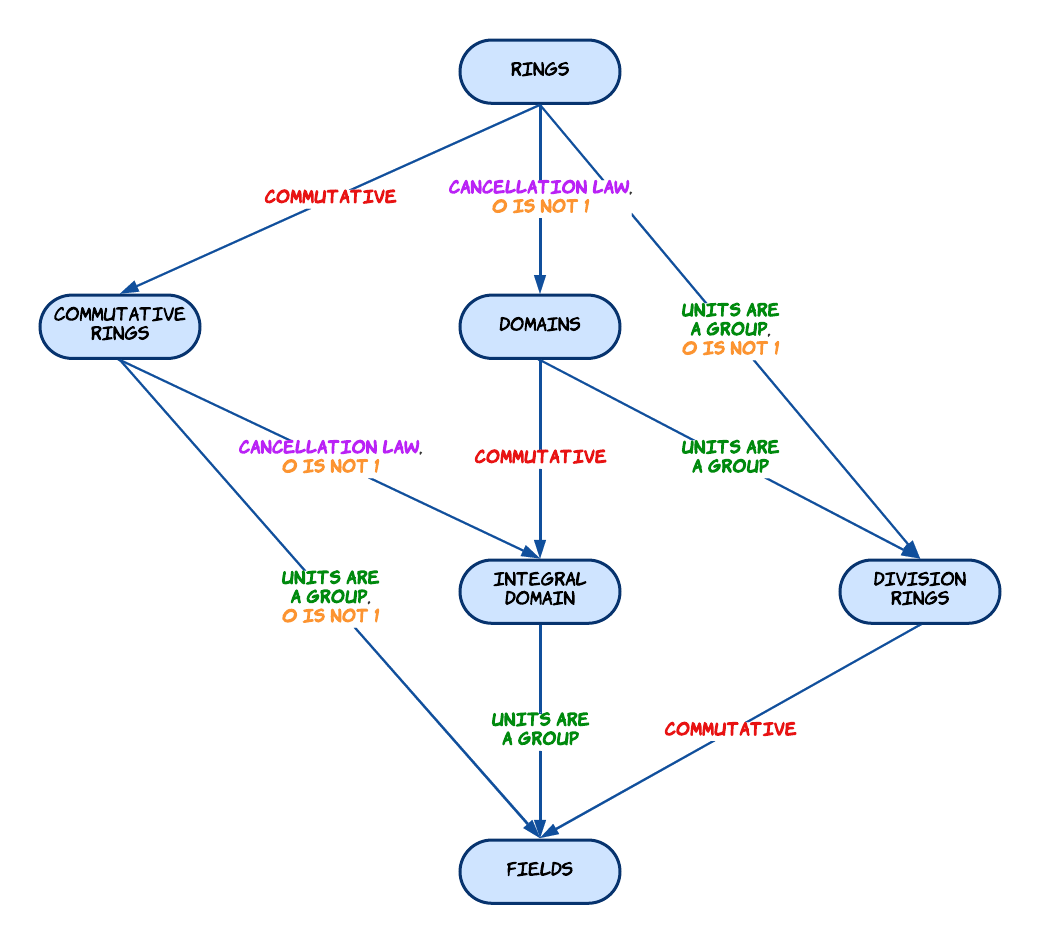
\includegraphics[scale = 0.3]{Ring Diagram}
\centering
\end{figure}

I like that there is a subtle sense of symmetry here. The conditions on the arrow is the condition for the ring in the tail to be a ring in the arrow head. For instance, if a domain $R$ satisfies the property that elements in $R$ are commutative, then $R$ is an integral domain. On the other hand, every integral domain will necessarily be a domain. 

\pagebreak
\subsection{Ring Homomorphisms and Ideals}
\begin{defn}{Ring Homomorphism}{} Let $R,S$ be rings. A ring homomorphism is a map $\phi:R\to S$ such that $$\phi(a+b)=\phi(a)+\phi(b)$$ and $$\phi(ab)=\phi(a)\phi(b)$$ for all $a,b\in R$. A bijective ring homomorphism is called a ring isomomorphism. 
\end{defn}

\begin{defn}{Kernel}{} The kernel of the ring homomorphism $\phi$, denoted $\ker(\phi)$ is defined as $$\ker(\phi)=\{r\in R|\phi(r)=0\}$$
\end{defn}

\begin{defn}{Ideals}{} Let $R$ be a ring. Let $I\subset R$ and let $r\in R$. Define $rI=\{ra|a\in I\}$ and $Ir=\{ar|a\in I\}$
\begin{itemize}
\item $I$ is a left ideal of $R$ if $(I,+)$ is a subgroup of $(R,+)$ and $rI\subseteq I$ for all $r\in R$
\item $I$ is a right ideal of $R$ if $(I,+)$ is a subgroup of $(R,+)$ and $Ir\subseteq I$ for all $r\in R$
\item A subset $I$ that is both a left ideal and right ideal is called an ideal of $R$. 
\end{itemize}
\end{defn}

\begin{lmm}{}{} Let $I$ be an ideal of a ring $R$. Then $I=R$ if and only if there exists a unit $u\in R$ such that $u\in I$. \tcbline
\begin{proof}
Let $I=R$. Then trivially $u\in I$. Now let $u\in I$ be a unit. Let $x\in R$, I want to show that $x\in I$ thus completing the proof that $R\subseteq I$. Now $x=x(u^{-1}u)=(xu^{-1})u$. Since $xu^{-1}\in R$ and $u\in I$, their muplication will also be in $I$, thus $x\in I$. 
\end{proof}
\end{lmm}

This lemma is also very useful if you consider the fact that the mupltiplicative identity is also a unit. 

\begin{prp}{}{} If $I,J$ are ideals of a ring $R$ then $$I+J=\{i+j|i\in I,j\in J\}$$ and $$I\cap J=\{r\in R|r\in I,r\in J\}$$ are both ideals of $R$. \tcbline
\begin{proof}
Let $R$ be a ring and $I,J$ its ideals. 
\begin{itemize}
\item We first show that $I+J$ is an ideal. Let $i_1+j_1,i_2+j_2\in I+J$. Then since $R$ is an abelian group an $I,J$ are subgroups of $R$, $$i_1+j_1+i_2+j_2=(i_1+i_2)+(j_1+j_2)\in I+J$$ thus closure is satisfied. Associativity is satisfied since it inherits from $R$. We also have $0\in I,J$ thus $0\in I+J$. The inverse of $i+j\in I+J$ is $-i-j\in I+J$ since $-i\in I$ and $-j\in J$. Thus $I+J$ is a subgroup of $R$. \\~\\
Now let $r\in R$ and $i+j\in I+J$. Then $r(i+j)=ri+rj$ by distributivity. Since $I,J$ are ideals, there exists $s\in I$ such that $s=ri$ and $t\in J$ such that $t=rj$. Then $r(i+j)=ri+rj=s+t\in I+J$ thus we are done. 
\item $I\cap J$ are already subgroups of $R$. Let $k\in I\cap J$. Let $r\in R$. Then $rk\in r(I\cap J)$. Then there exists $i\in I$ and $j\in J$ such that $i=rk=j$. Then $i=j\in I\cap J$ thus we are done. 
\end{itemize}
\end{proof}
\end{prp}

\begin{prp}{}{} The kernel of any ring homomorphism is an ideal. \tcbline
\begin{proof}
Kernels are trivially subgroups of $(R,+)$. Let $r\in R$. Let $x\in\ker(\phi)$. Then $\phi(rx)=\phi(r)\phi(x)=\phi(r)\cdot 0\in\ker(\phi)$ thus we are done. 
\end{proof}
\end{prp}

\begin{prp}{Quotient Ring}{} Let $I$ be an ideal of a ring $R$. Then the cosets of $I$ in $R$, $$R/I=\{r+I|r\in R\}$$ is a ring with addition defined the same as quotient groups $$(r+I)+(s+I)=(r+s)+I$$ and multiplication defined as $$(r+I)(s+I)=\{ab\in R|a\in r+I,b\in s+I\}=rs+I$$ called the quotient ring of $R$ by $I$. \tcbline
\begin{proof}
Since $(I,+)$ is a subgroup of $(R,+)$, we know that $R/I$ is already an abelian group. We simply show that multplication is well defined. Suppose that $x_1+I=x_2+I$ and $y_1+I=y_2+I$. Then 
\begin{align*}
(x_1+I)(y_1+I)&=x_1y_1+I\\
&=(x_1y_1-x_1y_2+x_1y_2-x_2y_2+x_2y_2)+I\\
&=(x_1(y_1-y_2)+(x_1-x_2)y_2+x_2y_2)+I\\
&=x_2y_2+I
\end{align*}
since $y_1-y_2\in I$ and $x_1-x_2\in I$. This shows that taking different represetatives of the cosets of an ideal does not matter for multiplication. \\~\\
Now we show that $1+I$ is the muplicative identity of $R/I$. Let $x+I\in R/I$. We have that $(1+I)(x+I)=x+I$ thus we are done. Associativity and distributivity follows from the fact that $R$ has these properties. 
\end{proof}
\end{prp}

\begin{thm}{}{} If $I$ is an ideal of $R$, the map $\phi:R\to R/I$ defined by $\phi(r)=r+I$ is a surjective ring homomorphism with kernel $I$. \tcbline
\begin{proof}
Let $a,b\in R$. Then 
\begin{align*}
\phi(a+b)&=(a+b)+I\\
&=(a+I)+(b+I)\\
&=\phi(a)+\phi(b)
\end{align*}
Now let $r\in R$. Then
\begin{align*}
\phi(ra)&=ra+I\\
&=(r+I)(a+I)\\
&=\phi(r)\phi(a)
\end{align*}
Now we show that $\phi$ is surjective. Let $r+I\in R/I$. Then trivially $\phi(r)=r+I$ thus we are done. \\~\\
Finally we show that $\ker(\phi)=I$. Let $a\in\ker(\phi)$. Then $\phi(a)=a+I=I$. This means that $a\in I$ and we have shown that $\ker(\phi)\subseteq I$. Now suppose that $a\in I$. Then $\phi(a)=a+I=I$. Thus $a\in\ker(\phi)$ and we are done. 
\end{proof}
\end{thm}

\subsection{Types of Ideals}
\begin{lmm}{}{} Let $R$ be a commutative ring and $a\in R$. Then $(a)=\{ar:r\in R\}$ is an ideal. \tcbline
\begin{proof}
Let $s,t\in(a)$. Then $s=ar_1$ and $t=ar_2$ for some $r_1,r_2\in R$. We show that $(a)$ is a subgroup of $R$. We have $$s+t=a(r_1+r_2)\in(a)$$ Identity is also in $(a)$ since $0\in R$ and $$a\cdot 0=0\in(a)$$ To show inverse we have that $u=-ar_1$ and $$s+u=ar_1-ar_1=0$$ By the subgroup criterion, $(a)$ is a group. We now show that $r(a)\subseteq(a)$. Let $r_1ar_2\in r(a)$. Then $$r_1ar_2=ar_1r_2\in(a)$$ since $R$ is commutative. Thus $(a)$ is an ideal. 
\end{proof}
\end{lmm}

\begin{defn}{Principal Ideals}{} Let $R$ be a commutative ring with identity. Let $I$ be an ideal of $R$. Then an ideal $I$ of the form $$I=(a)$$ for some $a\in I$ is called a principal ideal. 
\end{defn}

\begin{defn}{Maximal Ideals}{} A proper ideal $M$ of a ring $R$ is a maximal ideal of $R$ is the ideal $M$ is not a proper subset of any ideal of $R$ except $R$ itself. 
\end{defn}

Becareful that maximal ideals are not necessarily unique. A typical example would be the fact that $(2)$ and $(3)$ are principle ideals that are both maximal in $\Z$. 

\begin{defn}{Prime Ideals}{} A proper ideal $P$ in a commutative ring $R$ is called a prime ideal if $ab\in P$ implies $a\in P$ or $b\in P$. 
\end{defn}

\begin{prp}{}{} Let $R$ be a commutative ring with identity and $M$ an ideal of $R$. Then $M$ is maximal if and only if $R/M$ is a field. \tcbline
\begin{proof}
Suppose that $M$ is a maximal ideal. Let $x\notin R$. We show that $x+M$ has an inverse. We know that $M+(x)$ is an ideal containing $M$. Since $M$ is maximal, we must have $M+(x)=R$. This means that $1\in M+(x)$ which means there exists $m\in M$ and $r\in R$ such that $1=m+rx$. Now consider $r+M$. We have that 
\begin{align*}
(x+M)(r+M)&=xr+M\\
&=(1-m)+M\\
&=1+M
\end{align*}~\\
Now suppose that $R/M$ is a field. Let $J$ be an ideal such that $I\subseteq J\subseteq R$ and $I\neq J$. Now let $x\in J\setminus I$. Then $I+x$ has a multiplicative inverse in $R/I$ since $I+x\neq I$, the additive identity. Let the inverse be $I+y$. Then $$I+1=(I+x)(I+y)=I+xy$$ Trivially $xy\in(x)$, thus $1\in I+(x)\subseteq J$. But if the identity is in the ideal, the ideal is equal to the ring thus we are done. 
\end{proof}
\end{prp}

\begin{prp}{}{} Let $R$ be a commutative ring with identity not equal to $0$. Then $P$ is a prime ideal in $R$ if and only if $R/P$ is an integral domain. \tcbline
\begin{proof}
Suppose that $P$ is a prime ideal. Then let $(a+P)(b+P)=P$. Since we also have that $(a+P)(b+P)=ab+P$. This means that $ab\in P$ thus either $a\in P$ or $b\in P$ which in turns leads to either $a+P=P$ or $b+P=P$ and thus the cancellation law applies. \\~\\
Now suppose that $R/P$ is an integral domain. Let $ab\in P$. Since $R/P$ is an integral domain, we have that $$(a+P)(b+P)=ab+P=P$$ means that either $a+P=P$ or $b+P=P$ which means that either $a\in P$ or $b\in P$ and we are done. 
\end{proof}
\end{prp}

\begin{crl}{}{} Every maximal ideal in a commutative ring with identity is also a prime ideal. \tcbline
\begin{proof}
If $M$ is maximal then $R/M$ being a field implies that $R/M$ is an integral domain thus $M$ is prime. 
\end{proof}
\end{crl}

The proof is rather inconstructive in the sense that it does not provide a good insight to the structure, the reasoning behind why every maximal ideal is prime. For a more structure-revealing proof, consider the following alternative approach: \\~\\
Let $M$ be a maximal ideal of a commutative ring $R$. Let $ab\in M$ but $a\notin M$. Then $M+(a)=R$ since $M$ is maximal. Then $1\in R$ means that there exists $k\in M$ and $r\in R$ such that $k+ra=1$. Mutplying by $b$ gives $kb+rab=b$. Since $kb\in M$ and $rab\in M$, $b\in M$ and we are done. 

\pagebreak
\section{Integral Domains}
\subsection{Field of Fractions}
\begin{defn}{Fractional Equivalence}{} Let $R$ be an integral domain. Let $$S=\{(a,b)|a,b\in R\text{ and }b\neq 0\}$$ Define a relation on $S$ by $(a,b)\sim(c,d)$ if $ad=bc$. 
\end{defn}

\begin{lmm}{}{} The relation $\sim$ between elements of $S$ is an equivalence relation. \tcbline
\begin{proof}
Since $R$ is an integral domain, symmetry is satisfied. Clearly it is reflexive since $ab=ba$. For transitivity, suppose that $ad=bc$ and $cf=de$. Then $adcf=bcde$ and by cancellation law, $af=be$. 
\end{proof}
\end{lmm}

\begin{prp}{}{} The set of equivalence classes of $S$ of an integral domain $R$, under the equivalence relation $\sim$, together with the operations of addition and multiplication defined by $$(a,b)+(c,d)=(ad+bc,bd)$$ and $$(a,b)\cdot(c,d)=(ac,bd)$$ is a field, called the field of fractions, denoted $\text{Frac}(R)$. \tcbline
\begin{proof} Note that $R$ is a field if and only if $(R,+)$ and $(R\setminus\{0\},\cdot)$ are commutative groups and the distributive law holds. 
\begin{itemize}
\item Let $(a,b),(c,d)\in S$. Then $ad+bc,bd\in R$ since $R$ is closed thus $(ad+bc,bd)\in S$. Let $(e,f)$ also be in $S$. Then 
\begin{align*}
((a,b)+(c,d))+(e,f)&=(ad+bc,bd)+(e,f)\\
&=((ad+bc)f+(bd)e,bdf)\\
&=(adf+bcf+bde,bdf)
\end{align*}
and 
\begin{align*}
(a,b)+((c,d)+(e,f))&=(a,b)+(cf+de,df)\\
&=(a(df)+b(cf+de),b(df))\\
&=(adf+bcf+bde,bdf)
\end{align*}
Thus associativity is satisfied. I claim that $(0,1)$ is an identity. We have $(a,b)+(0,1)(a\cdot 1+b\cdot 0,b\cdot 1)=(a,b)$. If $(a,b)\in S$ then $(-a,b)\sim(a,-b)$ is an inverse. We have $$(a,b)+(-a,b)=(ab-ab,b^2)=(0,b^2)\sim(0,1)$$ Finally we have 
\begin{align*}
(a,b)+(c,d)&=(ad+bc,bd)\\
&=(da+cb,db)\tag{$R$ is an Integral Domain}\\
&=(cb+da,db)\tag{$R$ is an abelian group}
&=(c,d)+(a,b)
\end{align*}
Thus we have shown that $(S,+)$ is an abelian group. 
\item We now show that $(S,\cdot)$ is an abelian group. Let $(a,b),(c,d),(e,f)\in S$. Then $(a,b)\cdot(c,d)=(ac,bd)\in S$ sincve $ac,bd\in R$ by closure of rings. Thus the closure property is satisfied. Associativity is inherited from $R$ since elements in $S$ are pairs of $R$. I claim that the identity is $(1,1)\sim(k,k)$ for any $k\in R$. We have $$(a,b)\cdot(1,1)=(a\cdot1,b\cdot 1)=(a,b)$$ If $(a,b)\in S$ then its inverse is $(b,a)$. We have $$(a,b)\cdot(b,a)=(ab,ba)=(ab,ab)=(1,1)$$ thus $(S,\cdot)$ is a group. Now to show abelian, we have $$(a,b)\cdot(c,d)=(ac,bd)=(ca,db)=(c,d)\cdot(a,b)$$ since $R$ is an integral domain. Thus we have shown that $(S,\cdot)$ is an abelian group. 
\item Finally we show distributivity. Let $(a,b),(c,d),(e,f)\in S$. Then 
\begin{align*}
(a,b)\cdot((c,d)+(e,f))&=(a,b)\cdot(cf+de,df)\\
&=(acf+ade,bdf)
\end{align*}
and 
\begin{align*}
(a,b)\cdot(c,d)+(a,b)\cdot(e,f)&=(ac,bd)+(ae,bf)\\
&=(acbf+bdae,bdbf)\\
&=(acf+ade,bdf)\tag{equivalence relation}
\end{align*}
Thus we are done. 
\end{itemize}
\end{proof}
\end{prp}

In particular, the field of fractions of $\Z$ is precisely $\Q$. 

\begin{lmm}{}{} For any integral domain $R$, $R$ is a subring of $\text{Frac}(R)$. \tcbline
\begin{proof}
Define a function $\phi:R\to Q(R)$ by $\phi(r)=\frac{r}{1}$. Then $\phi_R$ is the identity homorphism thus $\phi(R)=R$. Then $\phi(R)$ is trivially a subring of $Q(R)$ and we are done. 
\end{proof}
\end{lmm}

\subsection{Divisibility}
\begin{defn}{Division}{} Let $R$ be a commutative ring and let $a,b\in R$ with $b\neq 0$. $a$ is said to be a multiple of $b$ if there exists an element $x\in R$ with $a=bx$. In this case $b$ is said to divide $a$ or be a divisor of $a$, written $b|a$. 
\end{defn}

\begin{prp}{}{} Let $R$ be a commutative ring. Let $x,y\in R$ and $y\neq 0$. Then the following are equivalent. 
\begin{itemize}
\item $x|y$
\item $y\in(x)$
\item $(y)\subseteq(x)$
\end{itemize}\tcbline
\begin{proof} Let $R$ be a commutative ring. Let $x,y\in R$ and $y\neq 0$. 
\begin{itemize}
\item $(1)\implies(2)$ Suppose that $y=kx=xk$ for some $k\in R$. Then $y\in(x)=\{ax|a\in R\}$ by definition. 
\item $(2)\implies(3)$ Suppose that $y\in(x)$. Then there exists $k\in R$ such that $y=kx=xk$. To show that $(y)\subseteq(x)$, let $ry\in(y)$. Then $ry=rkx$ and $rk\in R$ thus $ry\in(x)$ thus we are done. 
\item $(3)\implies(1)$ Suppose that $(y)\subseteq(x)$. Then there exists $k\in R$ such that $y=kx$. Then we are done. 
\end{itemize}
\end{proof}
\end{prp}

\begin{defn}{Greatest Common Divisor}{} A greatest common divisor of $a$ and $b$ is a non-zero element $d$ such that 
\begin{itemize}
\item $d|a$ and $d|b$
\item If $c|a$ and $c|b$ then $c|d$
\end{itemize} It is denoted $\gcd(a,b)$. 
\end{defn}

\begin{defn}{Least Common Multiple}{} A least common multiple of $a$ and $b$ is a non-zero element $l$ such that 
\begin{itemize}
\item $a|l$ and $b|l$
\item If $a|m$ and $b|m$ then $l|m$
\end{itemize} It is denoted $\lcm(a,b)$. 
\end{defn}

Unfortunately, these numbers do not always exists for any $a,b$ in a general ring. We will prove their existence in principal ideal domains later. 

\begin{prp}{}{} Let $R$ be a commutative ring. Let $x,y\in R$ such that they are nonzero. If the ideal generated by $a$ and $b$, namely $(a,b)$ is a principal ideal $(d)$, then $d$ is the gcd of $a$ and $b$. \tcbline
\begin{proof}
Suppose that $(a,b)=(d)$ for some $d\in R$. Then $a\in(d)$ and $b\in(d)$ already implies that $d|a$ and $d|b$. Suppose that $c|a$ and $c|b$. This means that $a\in(c)$ and $b\in(c)$. Since $d\in(a,b)$ there exists $r,s\in R$ such that $ra+sb=d$. This means that $d\in(c)$ thus $c|d$. 
\end{proof}
\end{prp}

This explains the notation that $(a,b)$ is often used to denote the gcd. 

\begin{defn}{Associates}{} Let $R$ be a commutative ring. Let $x,y\in R$. We say that $x$ and $y$ are associates if $x|y$ and $y|x$. We denote it as $x\sim y$. 
\end{defn}

\begin{prp}{}{} Let $R$ be a integral domain. Let $x,y\in R$. Then the following are equivalent. 
\begin{itemize}
\item $x\sim y$
\item $(x)=(y)$
\item There exists a unit $u\in R$ such that $x=qy$. 
\end{itemize} \tcbline
\begin{proof}
\begin{itemize}
\item $(1)\implies(2)$: Suppose that $x\sim y$ then $x|y$ and $y|x$ which means that $(x)\subseteq(y)$ and $(y)\subseteq(x)$. 
\item $(2)\implies(3)$: Suppose that $(x)=(y)$. Then since $x\in(y)$, there exists $s\in R$ such that $x=sy$ and likewise $y=tx$. Then $x=stx$ and since $R$ is an integral domain, $st=1$ which means that $s,t$ are units. 
\item $(3)\implies(1)$: Suppose that $x=qy$ for some unit $q$. Then clearly $y|x$. Since $q$ is a unit, $q^{-1}x=y$ and thus $x|y$ which means that $x$ and $y$ are associates. 
\end{itemize}
\end{proof}
\end{prp}

\subsection{Primes and Irreducibles}
Primes and irreducibles are two similar concepts, their difference is only made clear in Euclidean domains that are not principles ideal domains which we will see both notions later. 

\begin{defn}{Irreducibles}{} Let $D$ be an integral domain. A nonzero element $p\in D$ that is not a unit is said to be irreducible if $p=ab$ implies $a$ or $b$ is a unit. 
\end{defn}

\begin{defn}{Primes}{} Let $D$ be an integral domain. A nonzero element $p\in D$ that is not a unit is said to be a prime if $p|ab$ implies $p|a$ or $p|b$. 
\end{defn}

\begin{lmm}{}{} Let $D$ be an integral domain. Let $p$ be a non-unit. Then $p$ is prime if and only if $(p)$ is a prime ideal. \tcbline
\begin{proof}
Suppose that $p$ is prime. Suppose that $rp\in(p)$. Then $p\in P$ and we are done. Now suppose that $(p)$ is a prime ideal. Suppose that $p|ab$. Then $pd=ab$ for some $d\in D$ thus $ab\in(p)$. WLOG take $a\in(p)$ by definition of prime ideal. Then we are done since $a\in(p)$ implies $p|a$. 
\end{proof}
\end{lmm}

\begin{prp}{}{} Let $D$ be an integral domain and $p\in D$. If $p$ is a prime then $p$ is irreducible. \tcbline
\begin{proof}
Let $p$ be a prime in $D$. Suppose that $p=ab$. Then trivially $p|ab$ thus $p|a$ or $p|b$. WLOG take $p|a$. Trivially $a|p$ since $a|ab$. This means that $a$ and $p$ are associates. Thus $p=aq$ for some unit $q$. Then since $aq=ab$ and integral domains have cancellation law, we must have $q=b$ which means that $b$ is a unit. Thus $p$ is irreducible. 
\end{proof}
\end{prp}

\subsection{Unique Factorization Domains}
\begin{defn}{Unique Factorization Domains}{} An integral domain $D$ is a unique factorization domain if the following are true
\begin{itemize}
\item Let $a\in D$ such that $a\neq 0$ and $a$ is not a unit. Then $a$ can be written as the product of irreducible elements in $D$. 
\item Let $a=p_1\cdots p_r=q_1\cdots q_s$, where $p_i$ and $q_j$ are irreducible. Then $r=s$ and there is a permutation such that $p_i=q_{\pi(i)}$ for $i\in\{1,\dots,r\}$. 
\end{itemize}
\end{defn}

Notice that in general integral domains, primes are not the same as irreducibles. But they have the nice property that they coincide in UFDs, which is why they are put in the chapter on UFDs here. Below gives a full converse to the relation between prime and irreducibles we gave above under the umbrealla that is UFDs. 

\begin{prp}{}{} Let $D$ be a UFD and $p\in D$. Then $p$ is a prime if and only if $p$ is irreducible. \tcbline
\begin{proof}
We have already shown the forward implication. Now let $p$ be irreducible. We show that $(p)$ is prime. Let $ab\in(p)$. Then there exists $d\in D$ such that $pd=ab$. We can factorize $ab$ and $pd$ respectively into a product of irreducibles elements in $D$. But since they are equal, by uniqness of fatorization, $p$ is exactly an associate of one of the irreducibles in the factorization of $ab$. If $p$ is in the factorization of $a$ then $p|a$ and we are done. Otherwise it is in $b$ and we are also done. 
\end{proof}
\end{prp}

Notice that in the above proof, the fact that every prime is irreducible does not use the properties of UFD. This means that this is true in general integral domains. 

\subsection{Principal Ideal Domains}
\begin{defn}{Principal Ideal Domains}{} A principal ideal domain is an integral domain in which every ideal is principal, meaning every ideal is of the form $$(a)=\{ra:r\in R\}$$
\end{defn}

\begin{prp}{}{} Let $R$ be a PID and $x,y\in R$. Then $\gcd(x,y)$ and $\lcm(x,y)$ exists and there exists $r,s\in R$ such that $$\gcd(x,y)=rx+sy$$ \tcbline
\begin{proof}
Let $x,y\in R$. Then $(x)+(y)$ is an ideal of $R$, thus it must be prciniple, say $(d)=(x)+(y)$. Similarly, $(x)\cap(y)$ is also an ideal, say $(l)=(x)\cap(y)$. \\~\\
We prove that $d$ and $l$ are the gcd and lcm respectively. Trivially, $(x)\subseteq(d)$ and $(y)\subseteq(d)$ implies $d|x$ and $d|y$. Also for any $z$ such that $z$ divides $x$ and $y$, $(x)\subseteq(z)$ and $(y)\subseteq(z)$ thus $(d)\subseteq(z)$. The proof is similar for $(l)$. \\~\\
Since $(d)=(x)+(y)$, there exists $r,s\in (x),(y)$ respectively such that $d=rx+sy$ and we are done. 
\end{proof}
\end{prp}

\begin{prp}{}{} Let $R$ be a PID and $(p)$ a nonzero ideal in $R$. Then the following are equivalent. 
\begin{itemize}
\item $(p)$ is maximal
\item $p$ is irreducible
\item $p$ is prime ($(p)$ is prime)
\end{itemize} \tcbline
We have seen that every maximal ideal is a prime ideal. We have seen that if $(p)$ is a prime ideal then $p$ is prime. We have also seen that every prime is irreducible. We show separately that if $p$ is irreducible then $p$ is a prime, and also if $p$ is prime then $(p)$ is maximal. \\~\\
For the first part, suppose that $p$ is irreducible. Suppose that $p|ab$ for $a,b\in R$. By the above proposition, $d=\gcd(p,a)$ exists. Then for some $t\in R$, $p=dt$. Since $p$ is irreducible, either $d$ or $t$ is a unit. We consider both cases. If $t$ is a unit, then $p$ and $d$ are associates and thus $p|d$. Since $d|a$, we have that $p|a$ and we are done. Now if $d$ is a unit, then $d=ra+sp$ for some $r,s\in R$. Multplying both sides with $b$ gives $db=rab+spb$. Since $p|ab$ and $p|spb$, we have that $p|db$. Then $pu=db$ for some unit $u\in R$. Since $d$ is a unit, we have that $d^{-1}pu=b$, which means that $p|b$ and we are done. \\~\\
Now we show that if $p$ is a prime then $(p)$ is maximal. We know that $(p)$ is a prime ideal. Suppose that $(p)\subseteq(q)\subseteq R$ for some ideal $q$ of $R$. Since $p\in(q)$, $p=tq$ for some $t\in R$. Since $p\in(p)$, we have that $tq\in(p)$. Now $(p)$ is prime implies that either $t\in(p)$ or $q\in(p)$. If $q\in(p)$ then $(q)\subseteq(p)$ and thus $(q)=(p)$ and we are done. If $t\in(p)$, then $t=rp$ for some $r\in R$, which means that $p=rpq$. Then $rq=1$ by cancallation law in integral domains. This means that $1\in(q)$ thus $(q)=R$ and we are done. 
\end{prp}

\begin{prp}{}{} Every PID is a UFD. \tcbline
\begin{proof}
Suppose that $D$ is a principal ideal domain. Suppose for a contradiction that $x$, a non-unit cannot be factorized into a product of irreducibles. Clearly $x$ is not irreducible else a contradiction. Then there exists $x_1,y_1$ non unit such that $x=x_1y_1$. Since $x$ is assumed to be not a product of irreducibles, WLOG take $x_1$ to be not irreducible. Then we can repeat the process to get non units $x_2y_2$ such that $x_1=x_2y_2$. Notice that $(x)\subset(x_1)$ is a proper containment of ideals if $x_1|x$. Then we have a chain of ideals $$(x)\subset(x_1)\subset(x_2)\subset\dots$$ I claim that $$I=\bigcup_{k=0}^\infty(x_k)$$ is an ideal. Indeed if $r,s\in I$, then $r\in(x_m)$ and $s\in(x_n)$ for some $m,n\in\N$. WLOG rtake $m\leq n$. Then $(x_m)\subseteq(x_n)$ implies $r,s\in(x_n)$ thus $r+s\in(x_n)\subseteq I$. Also if $t\in R$, then $tr\in(x_m)\subseteq I$ thus $I$ is indeed an ideal. \\~\\
Since $R$ is a PID, there exists some $d\in I$ such that $I=(d)$. This also means that $d\in(x_m)$ for some $m\in\N$. Then this means that $I=(d)\subseteq(x_m)$. This proves that the chain eventually stops and this is a contradiction since we assumed that the chain of ideals are properly contained. \\~\\
This menas that $x$ can indeed be factorized into a product of irreducibles. 
\end{proof}
\end{prp}

Notice that the key in the proof is that the union of the countably finite principal ideals is again a principal ideals which allows the infinte chain of ideals to stop. 

\subsection{Euclidean Domains}
Technically, division algorithms can exist in general domains so long that it has the notion of division. But without a measurement of size to guarantee division is taking larger numbers into smaller numbers, we cannot promise that division algorithms will halt eventually. Therefore we restrict the notion of division algorithm only to integral domains that has a notion of size. 
\begin{defn}{Euclidean Valuation}{} Let $R$ be an integral domain. A function $f:R\setminus\{0\}\to\N\cup\{0\}$ is said to be a Euclidean Valuation of $R$ if
\begin{itemize}
\item $f(ab)\geq f(b)$ for all $a,b\in R\setminus\{0\}$
\item For all $a,b\in R$ with $b\neq0$, there exists $q,r$ such that $$a=qb+r$$ with $r=0$ or $f(r)<f(b)$
\end{itemize}
\end{defn}

In the above definition the second item is simply the division algorithm, with size of a number decided by the function $f$. Thus the Euclidean domain is simply an integral domain that possess a division algorithm. 

\begin{defn}{Euclidean Domain}{} An integral domain $R$ is said to be a Euclidean Domain that admits a Euclidean Valuation
\end{defn}

\begin{thm}{}{} Let $R$ be a Euclidean Domain. Let $a,b$ be nonzero elements of $R$. Let $d=r_n$ be the last nonzero remainder in the Euclidean Algorithm for $a$ and $b$. Then $d$ is the greatest common divisor of $a$ and $b$ and $(d)$ is generated by $a$ and $b$. In particular, there exists $x,y\in R$ such that $d=ax+by$. 
\end{thm}

\begin{prp}{}{} Every Euclidean Domain is a PID. 
\end{prp}

In general, we have that $$\text{Fields}\subset\text{Euclidean Domains}\subset\text{PID}\subset\text{UFD}\subset\text{Integral Domains}$$ in which all containments are strict. 

\pagebreak
\section{Polynomials}
\subsection{Polynomials over General Rings}
In this section we formulate the basic theory of generating polynomials from a ring. 
\begin{defn}{Indeterminates}{} Let $R$ be a ring. A symbol $x$ is called an indeterminate over $R$ if $$a_0+a_1x+a_2x^2+\dots+a_nx^n=0$$ where $a_i\in R$, implies that $a_i=0$ for each $i$. 
\end{defn}

\begin{defn}{Polynomial over a Ring}{} Any expression of the form $$f(x)=\sum_{k=0}^na_kx^k$$ where $x$ is an indeterminate and $a_0,\dots,a_n\in R$ and $a_n\neq 0$ is called a polynomial over $R$. We define the the degree of $f$ in this case to be $n$. 
\end{defn}

\begin{defn}{Ring of Polynomials}{} Let $R$ a ring. Define $R[x]$ to be the set of all polynomials over $R$. 
\end{defn}

\begin{prp}{}{} Let $R$ be a commutative ring with identity. Then $R[x]$ is a commutative ring with identity. \tcbline
\begin{proof}
Since $R\leq R[x]$ by considering all the constant polynomials, the identity of $R$ is also the identity of $R[x]$. Let $f,g\in R[x]$. Then the coefficient of $x^n$ in $f(x)g(x)$ is $$c_n=\sum_{k=0}^na_kb_{n-k}$$ Since $a_kb_{n-k}=b_{n-k}a_k$, we have that $f(x)g(x)=g(x)f(x)$. 
\end{proof}
\end{prp}

\begin{lmm}{}{} Let $R$ be a ring. Then $$\frac{R[x]}{(x)}\cong R$$ \tcbline
\begin{proof}
Taking the natural homomorphism $\phi:R[x]\to\frac{R[x]}{(x)}$ where $(x)$ is the ideal, we have that $\ker(\phi)=(x)$. By the first ring isomorphism theorem, $$\frac{R[x]}{(x)}\cong\phi(R[x])$$ But $\phi(R[x])$ is isomorphic to $R$ since every polynomial in $R[x]$ is a sum of a constant function and an element in $(x)$. 
\end{proof}
\end{lmm}

Whenever something similar to the above notion is seen, say $\frac{\Q[x]}{x-3}$, one can think of it as, whenever I see a factor of $x-3$ in $\Q[x]$, treat it as $0$. So if you want to find the image of $x^2-4x+5$ in the ring, we simply see that $x^2-4x+5=(x-3)(x-1)+2=2$ since $x-3$ is treated as $0$. Recalling that this is the quotient ring, we essentially quotient out all polynomials that has this factor which leads to $x^2-4x+5$ being treated as the same as the element $2$ in the ring. 

\begin{thm}{Evaluation Theorem}{} Let $R$ be a ring and let $a$ be an element in the center $Z(R)$ of $R$. Define a mapping $\phi_a:R[x]\to R$ by $$\phi_a\left(\sum_{k=0}^nc_kx^k\right)=\sum_{k=0}^nc_ka^k$$ Then $\phi_a$ is an onto ring homomorphism. 
\end{thm}

The evaluation maps gives a useful ring homomorphism to construct quotient rings. 

\subsection{Polynomials over Integral Domains}
\begin{prp}{}{} If $R$ is an integral domain then $R[x]$ is an integral domain. In particular the units in $R$ are also units in $R[x]$. \tcbline
\begin{proof}
Commutativity is clear since for $f,g\in R[x]$, coefficients of the product $fg$ inherits commutativity from $R$ thus $fg=gf$. Now we show that cancellation law exists in $R[X]$. Let $f,g\in R[x]$ such that $fg=0$. Suppose for a contradiction that $f\neq 0$ and $g\neq 0$. This means that $\deg(f)=n$ and $\deg(g)=m$ for some $n,m\neq 0$. Consider the coefficient of $x^{n+m}$ in $fg$, which is $a_nb_m$. Since $fg=0$, $a_nb_m=0$ and by cancellation law in $R$ either $a_n=0$ or $b_m=0$. This contradicts the fact that $\deg(f)=n$ and $\deg(g)=m$ thus we are done. \\~\\
The second part is trivial since $R\leq R[x]$ and they have the same identity. 
\end{proof}
\end{prp}

\begin{prp}{}{} Let $R$ be an integral domain. Then if $f\neq 0$ and $g\neq 0$ in $R[x]$, then $$\deg(fg)=\deg(f)+\deg(g)$$
\end{prp}

\begin{defn}{Irreducible Polynomial}{} Let $F$ be a field. A non constant polynomial $f\in F[x]$ is irreducible over $F$ if whenever $f(x)=g(x)h(x)$ with $g,h\in F[x]$, then one of $g$ or $h$ is a unit. 
\end{defn}

This defintion corresponds to the same definition of irreduciblesgiven in the UFD section. 

\subsection{Polynomials over UFDs}
The primary goal of this chapter is to compute results relating to finding out ireducible polynomials in UFD, rather than investigating the structure of polynomial rings. 
\begin{defn}{Primitive}{} An element $0\neq f\in R[x]$ where $R$ is a unique factorization domain is called primitive if $\gcd(a_0,a_1,\dots,a_n)=1$. 
\end{defn}

The reason that we have this notion is to prevent polynomials such as $5x-5$ to be discussed. This clearly will not be irreducible since there is a factor of $5$. Likewise if the gcd of all its coefficients are not $1$, then you can factor out the gcd from the entire polynomial. 

\begin{prp}{}{} The productive of two primitive polynomials is also primitive. 
\end{prp}

\begin{prp}{Eisentein's Criterion}{} Let $R$ be a UFD. Let $f\in R[x]$ be primitive. Suppose there is a prime $p\in R$ such that $p$ does not divide $a_n$ but $p|a_i$ for $0\leq i\leq n-1$ and $p^2$ does not divide $a_0$. Then $f$ is irreducible in $R[x]$. 
\end{prp}

\begin{thm}{}{} Let $R$ be a UFD with field of fractions $Q=Q(R)$. Then a primitive polynomial in $R[x]$ is irreducible if and only if it is irreducible in $Q[x]$. 
\end{thm}

An immediate corollary for when $R=\Z$ is as follows. 

\begin{thm}{Gauss' Lemma}{} A primitive irreducible polynomial in $\Z[x]$ remains irreducible in $\Q[x]$
\end{thm}

\begin{prp}{}{} $R$ is an UFD if and only if $R[x]$ is an UFD. 
\end{prp}

\subsection{Polynomials over a Field}
This section will mainly be revisiting old notations with $F[x]$. 
\begin{thm}{Division Algorithm}{} Let $F$ be any field and let $f$ and $g$ be polynomials in $F[x]$. Assume that $f\neq0$ and that the leading coefficient of $f$ is a unit in $R$. Then uniquely determined polynomials $q$ and $r$ exist in $F[x]$ such that 
\begin{itemize}
\item $g=qf+r$
\item Either $r=0$ or $\deg(r)<\deg(f)$
\end{itemize}
In particular, $\deg$ is an Euclidean Valuation of $F[x]$ and $F[x]$ is a Euclidean domain. 
\end{thm}

The above theorem is equivalent to saying that $F[x]$ is a Euclidean domain as long as $F$ is a field. Trivially, this also means that $F[x]$ is both a principal ideal domain and a unique factorization domain. \\~\\
We give an alternate proof showing that $F[x]$ is a principal ideal domain. \\~\\
Let $I$ be a nontrivial ideal of $F[x]$. Let $f\in I$ be nonzero such that the degree of $f$ is as small as possible. I claim that $(f)=I$. We already have that $(f)\subseteq I$ since $f\in I$. Now we show that $I\subseteq(f)$. So let $g\in I$. By the division algorithm, write $g=fq+r$ for some $q,r$ such that $\deg(r)<\deg(f)$ or $\deg(r)=0$. If $r\neq 0$, then $r=g-fq\in I$ since $f,g\in I$. But then $\deg(r)<\deg(f)$ means that $f$ is not of smallest degree in $I$, a contradiction. Thus $g=fq$, which means that $g\in(f)$. \\~\\
This is a constructive proof in the sense that if we would like to know the sole generator of an ideal in a polynomial ring $F[x]$ of a field, we simply take the polynomial of lowest degree. \\~\\

Since we have shown that polynomials over a field are euclidean domains, the following theorems and definitions are also trivial. 

\begin{lmm}{}{} Let $F$ be a field and suppose that $p\in F[x]$. Then the ideal generated by $p$ is maximal if and only if $p$ is irreducible. \tcbline
\begin{proof}
Proved when we introduced irreducibility. 
\end{proof}
\end{lmm}

\begin{prp}{Greatest Common Divisor}{} Let $f$ and $g$ be nonzero polynomials in $F[x]$, where $F$ is a field. Then a uniquely determined polynomial $d$ exists in $F[x]$ satisfying the following conditions. 
\begin{itemize}
\item $d$ is monic
\item $d$ divides both $f$ and $g$
\item If $h$ divides both $f$ and $g$, then $h$ divides $d$
\item $d=uf+vg$ for some polynomials $u,v\in F[x]$
\end{itemize}
\end{prp}

\begin{prp}{}{} Let $p\in F[x]$ be irreducible, $F$ a field. If $p$ divides a product $f_1f_2\cdots f_n$ of nonzero polynomials in $F[x]$, then $p$ divides one of $f_i$. 
\end{prp}

\begin{thm}{Unique Factorization Theorem}{} If $F$ is a field, let $f$ be a nonconstant polynomial in $F[x]$. Then 
\begin{itemize}
\item $f=ap_1p_2\cdots p_n$, where $a\in F$ and $p_i$ is monic and irreducible for all $i$
\item The factorization is unique up to the order of the factors
\end{itemize}
\end{thm}

We now begin dicussion of new notions that only polynomial rings based on a field will have. 

\begin{thm}{Factor Theorem}{} Let $F$ be a field. Let $a\in R$. Let $f\in F[x]$. Then $f(a)=0$ if and only if $f=(x-a)q$ for some $q\in F[x]$. \tcbline
\begin{proof}
Clearly if $f$ is of the form $f=(x-a)q$ then $f(a)=0$. \\~\\
Now suppose that $f(a)=0$. We apply the division algorithm on $f$ with $x-a$ to get $$f(x)=(x-a)q(x)+r(x)$$ where either $r(x)=0$ or $\deg(r)<1$. This means that $r(x)=k$ for some constant $k\in F$. Since $f(a)=0$, we have that $(a-a)q(a)+k=0$ which means that $k=0$ and we are done. 
\end{proof}
\end{thm}

\begin{prp}{}{} Let $F$ be a field and let $f$ be a nonzero polynomial in $F[x]$ of degree $n$. Then $f$ has at most $n$ roots in $R$. 
\end{prp}

\begin{thm}{Remainder Theorem}{} Let $F$ be a field. Let $a\in F$. Let $f\in F[x]$. If $f$ is divided by $(x-a)$, the remainder is $f(a)$. \tcbline
\begin{proof}
By division algorithm, there exists $q,r\in F[x]$ such that $f(x)=(x-a)q(x)+r(x)$. Evaluating $x$ at $a$ gives $f(a)=r(a)$. 
\end{proof}
\end{thm}

\subsection{Number Fields}
This section to be removed to Field Theory. 
\begin{defn}{Algebraic Elements}{} Let $\alpha\in\C$. We say that $\alpha$ is algebraic over $\Q$ if there exists $f\in\Q[x]$ such that $f(\alpha)=0$ where $f$ is not the identity. Otherwise $\alpha$ is said to be transcendental. 
\end{defn}

\begin{prp}{}{} If $\alpha$ is an algebraic element of $\C$, then there exists a unique nonzero irreducible polynomial $f\in\Q[x]$ with leading coefficient $1$ such that $f(\alpha)=0$. 
\end{prp}

Using the first isomorphism theorem for rings, we se that the image of the evaluation map $$\im(\phi_\alpha)\cong\Q[x]/(f)$$ Since $f$ is irreducible, $\Q[x]/(f)$ is a field, called a number field. 

\begin{defn}{Number Fields}{} For any $\alpha\in\C$ an algebraic element, we define $$\Q[\alpha]=\Q[x]/(f)$$ to be the number field containing $\alpha$. 
\end{defn}

Let us look at an example. \\~\\
Suppose we want to quotient out the polynomial $x^2-4x+3$ in $\Q[x]$. Then notice that $3$ and $1$ are roots of the quadratic. So we have that $$\Q[x]/(x-3)\cong\phi_3(\Q[x])$$ where $\phi_3$ is the evaluation map at $3$. This is proven as follows: We show that $\ker(\phi_3)=(x-3)$ the ideal and thus we can apply the first ring isomorphism theorem. \\~\\
Suppose that $f\in\ker(\phi_3)$. Then $f(3)=0$ and since $f\in\Q[x]$, $f$ has a linear factor $x-3$ by by division algorithm which we will see later. Then $f\in(x-3)$. Now if $g\in(x-3)$, then $g(x)=(x-3)f(x)$ for some $f\in\Q[x]$ and clearly $g(3)=0$. Thus $\ker(\phi_3)=(x-3)$. \\~\\
Now we reapply the first ring isomorphism theorem which the evaluation map $$\phi_1:\frac{\Q[x]}{(x-3)}\to\Q$$ with the same method and we get $$\frac{\Q[x]}{(x-3)(x-1)}\cong\phi_1(\phi_3(\Q[x]))$$


\pagebreak
\section{Important Rings to Note}
\subsection{The Number Fields $\Z$, $\Q$, $\R$ and $\C$ and its Polynomial Rings}
\begin{thm}{}{} The number fields $\Z$, $\Q$, $\R$ and $\C$ are all commutative rings with identity. In particular, 
\begin{itemize}
\item $\Q$, $\R$, $\C$ are Fields
\item $\Z$ is an Euclidean Domain
\end{itemize}
\end{thm}

\begin{lmm}{}{} The field of fractions of $\Z$ is equivalent to $\Q$. Meaning $Q(\Z)=\Q$. 
\end{lmm}

\subsection{The Modulo Rings $\Z/n\Z$ and the Finite Fields $\F_p$}
\begin{thm}{}{} The modulo rings $\Z/n\Z$ is a quotient ring that is commutative with kernel $n\Z$. 
\end{thm}

\begin{thm}{}{} $\Z/p\Z$ is a field with characteristic $p$ if and only if $p$ is a prime. 
\end{thm}

\subsection{The Matrix Groups $GL(n,F)$, $SL(n,F)$ and $O(n)$}
\begin{thm}{The Matrix Groups}{} Let $F$ be a field. Denote $GL(n,F)$ the set of all $n\times n$ matrices over $F$ with nonzero determinant, called the general linear group, is a group. $SL(n,F)$, the special linear group, defined to be $$SL(n,F)=\{M\in GL(n,F)|\det(M)=1\}$$ is a subgroup of $GL(n,F)$. The orthogonal group, defined to be $$O(n)=\{M\in GL(n,F)|M^TM=MM^T=I\}$$ is a subgroup of $SL(n,F)$. 
\end{thm}

\begin{lmm}{}{} Let $F$ be a field. Check that $O(n)\leq SL(n,F)\leq GL(n,F)$. 
\end{lmm}
